\documentclass[a4paper,12pt]{article}

% 中文支持
\usepackage{xeCJK}
\usepackage{fontspec}
\setCJKmainfont{SimSun}
\setCJKsansfont{SimHei}
\setCJKmonofont{SimSun}

% 标题全部使用黑体（\sffamily）
\usepackage{titlesec}
\titleformat{\section}{\Large\bfseries\sffamily}{\thesection}{1em}{}
\titleformat{\subsection}{\large\bfseries\sffamily}{\thesubsection}{1em}{}
\titleformat{\subsubsection}{\normalsize\bfseries\sffamily}{\thesubsubsection}{1em}{}

% 页面设置
\usepackage{geometry}
\geometry{left=2.5cm,right=2.5cm,top=2.5cm,bottom=2.5cm}

% 数学与符号
\usepackage{amsmath,amssymb,amsfonts}

% 图表
\usepackage{graphicx}
\usepackage{booktabs}
\usepackage{multirow}
\usepackage{array}
\usepackage{float}
\usepackage{caption}
\usepackage{subcaption}

% 颜色与高亮
\usepackage{xcolor}
\usepackage{listings}
\lstset{
 basicstyle=\ttfamily\small,
 keywordstyle=\color{blue},
 commentstyle=\color{green!50!black},
 stringstyle=\color{red!60!black},
 numbers=left,
 numberstyle=\tiny,
 breaklines=true,
 frame=single,
 columns=flexible,
 showspaces=false,
 showstringspaces=false,
}

% 超链接
\usepackage{hyperref}
\hypersetup{colorlinks=true,linkcolor=blue,citecolor=blue,urlcolor=blue}

% 参考文献
\usepackage[numbers,super,sort&compress]{natbib}

% 算法
% \usepackage{algorithm}
% \usepackage{algorithmic}

% 其他
\usepackage{enumitem}
\usepackage{tikz}
\usetikzlibrary{shapes,arrows,positioning}

% 行距
\usepackage{setspace}
\onehalfspacing

% 页眉页脚
\usepackage{fancyhdr}
\pagestyle{fancy}
\fancyhf{}
\fancyhead[C]{\small\sffamily 地书图形语言与自然语言的象似性与组合性对比研究}
\fancyfoot[C]{\thepage}
\renewcommand{\headrulewidth}{0.4pt}

\begin{document}

% ==================== 标题页 ====================
\begin{titlepage}
\centering
\vspace*{2cm}
{\LARGE\bfseries\sffamily 从象似性与组合性视角看《地书》图形语言\\[0.3cm]与自然语言的异同}\\[1.5cm]
{\large A Comparative Study of Iconicity and Compositionality\\between the ``Earth Book'' Graphic Language and Natural Language}\\[2cm]
{\large 《自然语言处理》课程论文}\\[1cm]
\vspace{2cm}
\vfill
\vspace{1cm}
\end{titlepage}

% ==================== 摘要 ====================
\newpage
\section*{摘要}
\addcontentsline{toc}{section}{摘要}

《地书》（Earth Book）是由徐冰创作的一套完全由图形符号构成的叙事系统，其以象形图形替代文字进行表达，在视觉上具有高度的象似性（iconicity），但其组合方式是否遵循自然语言的句法规律仍是一个开放的研究问题。本文从\textbf{象似性}与\textbf{组合性}两个核心语言学维度出发，对《地书》的图形标注数据（材料1）和白话文本标注数据（材料2）进行了系统的对比分析，并结合古典汉语（四库全书）、现代新闻（THUcNews）、小说及世界名著等多种自然语言语料库（材料3）作为参照。

研究方法涵盖了Transformer以前的经典NLP技术（词频统计、N-gram分析、TF-IDF、分布对比）以及基于Transformer的大语言模型方法（BERT中文预训练模型的语义嵌入分析）。实验结果表明：（1）《地书》图形在词性层面表现出显著的``标点/边界标记''偏好（32.3\%），远超自然语言文本的标点比例，反映了图形系统的空间边界依赖；（2）地书图形的语义基元以``运动''、``情感''、``人类''为主，与自然语言词汇的语义分布存在结构性差异；（3）篇章关系以``时间先后''（43.7\%）和``因果''（17.9\%）为主导，体现了图形叙事的强时序性；（4）BERT嵌入分析显示，地书图形的字面释义（literal gloss）具有内部语义一致性（组内相似度0.770），但跨组泛化能力略低于白话文本（0.762 vs 0.786），表明图形到语言的映射仍具有一定的非系统性。

\textbf{关键词：}地书；图形语言；象似性；组合性；计算语言学；BERT；对比分析

\vspace{0.5cm}
\noindent\textbf{Abstract:} This paper investigates the similarities and differences between Xu Bing's ``Earth Book'' graphic language and natural language from the perspectives of iconicity and compositionality. Through systematic analysis of annotated graphic data (Material 1), vernacular text annotations (Material 2), and multiple natural language corpora (Material 3), we employ both classical NLP methods and Transformer-based BERT embeddings. The results reveal distinctive structural properties of the graphic language, including its spatial boundary dependency, event-driven semantic primitives, and strong temporal sequentiality in discourse relations.

\textbf{Keywords:} Earth Book; Graphic Language; Iconicity; Compositionality; Computational Linguistics; BERT; Comparative Analysis

% ==================== 目录 ====================
\newpage
\tableofcontents
\newpage

% ==================== 1. 引言 ====================
\section{引言}\label{sec:intro}

\subsection{研究背景}

语言的本质特征长期以来被索绪尔（Saussure）定义为``任意性''（arbitrariness）——即语言符号的能指与所指之间不存在自然的、必然的关联\cite{saussure1916}。然而，皮尔斯（Peirce）的符号三元理论指出，符号可分为图像符（icon）、指示符（index）和象征符（symbol），其中图像符的能指与所指之间存在象似性（iconicity）关系\cite{peirce1931}。自然语言中，拟声词、象形文字（如汉字）以及某些手势语言均表现出不同程度的象似性。

《地书》（英文名：\textit{Book from the Ground}）是中国艺术家徐冰自2003年起创作的一套叙事作品\cite{xubing2012}。与传统文字系统不同，《地书》完全依赖从公共场所标识、交通标志、商业符号、网络表情等日常视觉符号中选取和重组的图形元素进行叙事。这些图形元素在视觉上与其所代表的概念高度相似——例如，一个奔跑的小人表示``跑''或``逃跑''，一个笑脸表示``开心''或``友好''。因此，《地书》构成了一个天然的``高象似性语言系统''实验样本。

与此同时，象似性并非语言理解的唯一维度。组合性（compositionality）——即整体意义由其组成部分的意义及组合规则决定——被认为是人类语言理解的核心机制之一\cite{frege1892,montague1970}。自然语言通过句法规则将词汇组合成短语和句子，使得人类能够理解从未见过的新表达。《地书》的图形序列是否也遵循类似的组合性原则？一组图形整体的意义是否可以从其组成部分的图形意义和排列顺序中推导出来？这些问题构成了本文的研究核心。

\subsection{研究问题}

基于上述背景，本文提出以下研究问题：

\begin{enumerate}[label=\textbf{RQ\arabic*:},leftmargin=2cm]
    \item 《地书》图形的象似性程度在语言学标注中表现出何种分布特征？与古典汉语、现代汉语新闻及小说的词汇分布有何异同？
    \item 《地书》图形组合的组合性程度如何？其分组结构（groups）是否表现出类似自然语言短语/句子的层级组织？
    \item 经典NLP方法（统计、N-gram、TF-IDF）与Transformer方法（BERT语义嵌入）在刻画《地书》与自然语言的异同方面各有何优势？
    \item 《地书》的``篇章关系''（discourse relation）分布反映了图形叙事的何种认知特征？
\end{enumerate}

\subsection{研究意义}

本研究的意义体现在以下三个层面：

\textbf{理论层面}：本研究为``图形语言是否属于语言''这一跨学科论题提供了计算语言学的实证数据。通过将《地书》置于与自然语言相同的标注框架下进行多维比较，我们得以在统一的分析维度上检验图形语言是否满足语言学的核心特征。

\textbf{方法层面}：本文同时采用经典NLP方法和基于Transformer的深度学习方法，展示了两种方法论在分析非传统语言材料时的互补性。特别是BERT嵌入分析为量化图形的语义一致性提供了新的技术手段。

\textbf{应用层面}：对《地书》的结构化分析可为象形文字识别、视觉符号理解、跨模态翻译（图像到文本）以及辅助沟通系统（AAC）的设计提供语言学依据。

% ==================== 2. 相关工作 ====================
\section{相关工作}\label{sec:related}

\subsection{图形语言与视觉符号系统}

图形语言的研究可追溯至Bliss符号系统（Blissymbolics）和人类的史前洞穴壁画。Bliss于1949年提出的Blissymbolics是一套由逻辑图形构成的辅助沟通系统，其设计目标是实现跨语言的可理解性\cite{bliss1965}。与Blissymbolics的人工设计不同，《地书》的图形来源于现成的社会视觉符号，因此具有更强的文化嵌入性和约定性（conventionality）。

在语言学领域，McNeill\cite{mcneill1992}对手势语言的研究表明，手势与言语共享同一套认知-语言系统，手势的象似性（iconicity）并不影响其组合性（compositionality）。类似地，美国手语（ASL）的研究表明，即使高度象似的手势，一旦进入语法系统，其组合方式仍然遵循严格的句法规则\cite{klima1979}。这些发现为理解《地书》的组合性提供了理论参照。

\subsection{象似性与组合性的理论框架}

象似性在语言学中通常被操作化为``形式与意义之间的结构对应''\cite{haiman1985}。Givón\cite{givon1985}提出了象似性的多个维度，包括距离象似性（distance iconicity）、数量象似性（quantity iconicity）和顺序象似性（sequential iconicity）。《地书》的图形排列顺序显然遵循顺序象似性原则——事件的先后关系直接映射为图形的空间先后关系。

组合性的形式化定义通常借助类型论和λ演算\cite{montague1970}。在计算语言学中，组合性可以通过分布语义学（distributional semantics）来近似衡量——如果复合表达式的语义向量与其组成部分的语义向量存在可预测的组合函数关系，则可认为该系统具有较高组合性\cite{mitchell2010}。本文采用BERT嵌入向量的余弦相似度作为语义一致性的量化指标，以此间接衡量组合性。

\subsection{计算语言学中的多模态分析}

近年来，多模态学习（multimodal learning）领域出现了大量将视觉信息与语言信息进行联合建模的工作。CLIP\cite{radford2021}和ALIGN\cite{jia2021}等模型通过对比学习实现了图像与文本的联合嵌入空间。然而，这些工作主要关注自然图像与描述性文本的对应关系，而非系统性的图形语言。《地书》作为一套有完整叙事结构的人工图形语言，为多模态研究提供了一个独特的受控实验样本。

% ==================== 3. 数据与方法 ====================
\section{数据与方法}\label{sec:method}

\subsection{数据来源与预处理}

本研究使用了三类数据材料，共计约3GB文本及图形标注数据：

\subsubsection{材料0：人工标注系统}

《地书》标注系统V1.0是一个纯前端（Vanilla JS）的数据标注工具，核心文件包括：
\begin{itemize}
    \item \texttt{app.js}：核心业务逻辑，支持Grouping（多级分组）和Labeling（多任务标注）两种模式
    \item \texttt{data/segments\_manifest.js}：12,078个原子图形（Atom）数据清单
    \item \texttt{data/config.js}：22个标注任务的动态配置
\end{itemize}

标注系统的数据模型包含三类核心对象：
\begin{enumerate}
    \item \textbf{Atom}：最小图形单元，属性包括全局排序号（\texttt{global\_order}）、页码（\texttt{page\_no}）、左右页（\texttt{side}：L/R）、行号（\texttt{line\_no}）、宽高（\texttt{width}, \texttt{height}）
    \item \textbf{Group}：分组对象，由连续的Atom或子Group组成，支持多级嵌套（\texttt{level}层级）
    \item \textbf{Annotation}：标注数据，绑定到Atom或Group，包含任务ID（\texttt{task\_id}）和标注值（\texttt{value}）
\end{enumerate}

系统导出的标准JSON格式包含：\texttt{project}、\texttt{config\_snapshot}、\texttt{session}（标注者信息及页码范围）、\texttt{groups}、\texttt{annotations}。

\subsubsection{材料1：《地书》基础词/句标注数据}

材料1包含365个有效的词标注文件和342个句标注文件，文件名为\texttt{地书-词标注 (编号).txt}。标注内容覆盖以下主要维度：
\begin{itemize}
    \item \textbf{字面对应词}（\texttt{literal\_gloss}）：7,066条，记录图形最直接的自然语言对应词
    \item \textbf{词性/符号性质}（\texttt{pos\_like\_category}）：6,728条，多选标签（名词性、动词性、形容词性、标点/边界标记等）
    \item \textbf{类形态特征}（\texttt{morphological\_features}）：5,332条（词标注）+ 2,025条（句标注），多选标签（进行体、现在时、否定、强调等）
    \item \textbf{语义基元}（\texttt{semantic\_primitives}）：1,561条（词标注）+ 770条（句标注），多选标签（人类、有生命、运动、情感、空间等）
    \item \textbf{语境实际含义}（\texttt{pragmatic\_meaning}）：5,121条（词标注）+ 1,321条（句标注）
    \item \textbf{篇章关系}（\texttt{discourse\_relation}，仅句标注）：4,847条，单选标签（时间先后、因果、并列递进、解释说明等）
\end{itemize}

\subsubsection{材料2：《地书》白话版标注数据}

材料2包含192个有效的白话版词标注文件，采用与材料1相同的标注维度，但标注对象为自然语言文本（非图形）。每个文件包含：\texttt{project}（项目信息）、\texttt{student}（标注者信息）、\texttt{source\_text}（白话文本内容）、\texttt{units}（标注单元列表，含\texttt{id}和\texttt{token}）、\texttt{annotations}（标注结果列表）。

材料2的关键价值在于提供了\textbf{同一套标注框架}下图形与文本的直接可比性。

\subsubsection{材料3：对比语料库}

本研究选取了五类自然语言语料作为对比基准：
\begin{enumerate}
    \item \textbf{四库全书数据库}（殆知阁汉语古文数据集）：10大类别（易藏、儒藏、道藏、佛藏、子藏、史藏、诗藏、集藏、医藏、艺藏），古典汉语
    \item \textbf{世界名著}（现代中文翻译）：现代汉语翻译文学
    \item \textbf{THUcNews}：现代汉语新闻语料，含训练集（4,500条）、验证集（400条）、测试集（900条）
    \item \textbf{小说}：现代中文通俗小说，约1,145万行
    \item \textbf{WikiSentences30k\_16Lans}：16种语言各30,000句的维基百科句子集，含中文子集
\end{enumerate}

\subsection{数据预处理与解析}

本节介绍数据处理的技术细节。所有代码使用Python 3.12实现，依赖库包括\texttt{json}、\texttt{glob}、\texttt{pandas}、\texttt{numpy}、\texttt{scikit-learn}、\texttt{transformers}和\texttt{torch}。

\subsubsection{JSON标注文件加载与解析}

材料1和材料2的标注数据以JSON格式存储，每个文件对应一个标注者在一个页码范围内的标注结果。由于标注者输入可能存在编码问题或空文件，数据加载过程需要进行异常处理。代码~\ref{code:load}展示了核心的JSON文件加载函数，该函数遍历指定目录下的所有\texttt{.txt}文件，对非空且格式正确的JSON文件进行解析，并返回文件路径与数据字典的配对列表。

\begin{lstlisting}[language=Python, caption=JSON标注文件加载函数, label=code:load]
import json, glob
from pathlib import Path

def load_json_files(path_pattern):
    """加载所有JSON文件，忽略编码错误和空文件"""
    files = glob.glob(path_pattern)
    valid = []
    for f in files:
        try:
            with open(f, 'r', encoding='utf-8') as fp:
                raw = fp.read().strip()
                if not raw: 
                    continue
                data = json.loads(raw)
            if isinstance(data, dict) \
               and isinstance(data.get('annotations'), list):
                valid.append((f, data))
        except:
            pass
    return valid
\end{lstlisting}

\subsubsection{标注维度提取}

在加载原始JSON文件后，需要将标注数据按\texttt{target\_id}（被标注对象）和\texttt{task\_id}（标注任务类型）进行重组，以便进行后续的统计分析与对比。代码~\ref{code:extract}展示了按目标对象聚合标注维度的核心逻辑。该函数为每个\texttt{target\_id}建立任务维度到标注值的映射字典，支持从材料1（图形标注）和材料2（文本标注）中统一提取信息。

\begin{lstlisting}[language=Python, caption=标注维度按目标对象聚合提取, label=code:extract]
from collections import defaultdict

def extract_annotations_by_target(data):
    """将annotations按target_id聚合"""
    target_anns = defaultdict(dict)
    for ann in data.get('annotations', []):
        tid = ann['target_id']
        task = ann['task_id']
        target_anns[tid][task] = ann['value']
    return target_anns

def extract_flat_values(records, task_id):
    """从所有记录中提取某task的flat值列表"""
    values = []
    for _, data in records:
        for ann in data.get('annotations', []):
            if ann.get('task_id') == task_id:
                v = ann.get('value')
                if isinstance(v, list):
                    values.extend([str(x) for x in v if x])
                elif v is not None and str(v).strip():
                    values.append(str(v))
    return values
\end{lstlisting}

\subsubsection{分组结构解析}

材料1的分组（\texttt{groups}）数据记录了标注者创建的图形组合单元，每个分组包含层级（\texttt{level}）、子节点列表（\texttt{children}）以及覆盖的Atom起止范围（\texttt{leaf\_start}、\texttt{leaf\_end}）。代码~\ref{code:group}展示了分组结构的核心解析逻辑，用于计算层级分布和组大小统计。

\begin{lstlisting}[language=Python, caption=分组结构解析与统计, label=code:group]
import numpy as np
from collections import Counter

def analyze_groups(data):
    """解析分组结构并返回统计指标"""
    level_counter = Counter()
    group_sizes = []
    for g in data.get('groups', []):
        level = g.get('level', 0)
        level_counter[level] += 1
        size = g['leaf_end'] - g['leaf_start'] + 1
        group_sizes.append(size)
    return {
        'total': sum(level_counter.values()),
        'level1': level_counter.get(1, 0),
        'level2plus': sum(v for k, v in level_counter.items() 
                          if k >= 2),
        'mean_size': np.mean(group_sizes) if group_sizes else 0,
        'median_size': np.median(group_sizes) if group_sizes else 0,
    }
\end{lstlisting}

\subsection{经典NLP分析方法}

\subsubsection{描述性统计与分布对比}

对材料1和材料2的各标注维度进行频次统计和百分比计算，重点对比以下分布：
\begin{itemize}
    \item POS-like category分布（图形 vs 文本）
    \item Semantic primitives分布（图形 vs 文本）
    \item Morphological features分布（图形 vs 文本）
    \item Discourse relation分布（仅句标注）
\end{itemize}

\subsubsection{TF-IDF与区分性词汇分析}

使用scikit-learn的\texttt{TfidfVectorizer}对地书图形的\texttt{literal\_gloss}和白话文本的\texttt{literal\_gloss}进行TF-IDF向量化，提取两组中最具区分性的特征词（discriminative words），以揭示图形释义与文本释义的语义焦点差异。具体实现中，首先对两组各500条字面释义进行中文分词（正则提取连续中文字符串），然后合并为统一语料库进行TF-IDF向量化，最后计算两组在各特征词上的平均TF-IDF得分差异，提取差异最大的20个特征词作为区分性词汇。TF-IDF的计算公式为：
\begin{equation}
    \text{TF-IDF}(t, d) = \text{tf}(t, d) \times \text{idf}(t)
\end{equation}
其中$\text{tf}(t, d)$为词$t$在文档$d$中的词频，$\text{idf}(t) = \log \frac{N}{|\{d : t \in d\}|}$为逆文档频率。代码~\ref{code:tfidf}展示了TF-IDF区分性词汇提取的核心实现。

\begin{lstlisting}[language=Python, caption=TF-IDF区分性词汇分析, label=code:tfidf]
import re, numpy as np
from sklearn.feature_extraction.text import TfidfVectorizer

def tokenize(texts):
    """提取中文字符串作为token"""
    docs = []
    for t in texts:
        words = re.findall(r'[\u4e00-\u9fff]{2,}', t)
        docs.append(' '.join(words))
    return docs

def analyze_tfidf_distinctive(gloss1, gloss2, top_n=20):
    docs1 = tokenize(gloss1)
    docs2 = tokenize(gloss2)
    corpus = docs1 + docs2
    labels = ['dishu'] * len(docs1) + ['baihua'] * len(docs2)
    
    vectorizer = TfidfVectorizer(max_features=200, min_df=2)
    tfidf_matrix = vectorizer.fit_transform(corpus)
    feature_names = vectorizer.get_feature_names_out()
    
    dishu_idx = [i for i, l in enumerate(labels) if l == 'dishu']
    baihua_idx = [i for i, l in enumerate(labels) if l == 'baihua']
    
    dishu_mean = np.array(tfidf_matrix[dishu_idx].mean(axis=0)).flatten()
    baihua_mean = np.array(tfidf_matrix[baihua_idx].mean(axis=0)).flatten()
    
    diff = dishu_mean - baihua_mean
    top_dishu = np.argsort(diff)[-top_n:][::-1]
    top_baihua = np.argsort(diff)[:top_n]
    
    return [feature_names[i] for i in top_dishu], \
           [feature_names[i] for i in top_baihua]
\end{lstlisting}

\subsubsection{分组结构分析}

对材料1中的\texttt{groups}数据进行结构统计，包括层级分布（Level 1 vs Level 2+）、组大小分布（覆盖的Atom数量）和子节点数量分布。分组数据以JSON数组形式存储，每个分组对象包含以下关键字段：\texttt{id}（唯一标识）、\texttt{level}（层级深度）、\texttt{children}（子节点ID列表）、\texttt{leaf\_start}和\texttt{leaf\_end}（覆盖的Atom起止全局排序号）。组大小通过\texttt{leaf\_end $-$ leaf\_start $+$ 1}计算，层级通过统计\texttt{level}字段的频次分布获得。代码~\ref{code:groupstat}展示了分组结构统计的核心实现。

\begin{lstlisting}[language=Python, caption=分组结构统计, label=code:groupstat]
from collections import Counter
import numpy as np

def analyze_group_structure(records):
    """对材料1的所有groups进行结构统计"""
    level_counter = Counter()
    group_sizes = []
    
    for _, data in records:
        for g in data.get('groups', []):
            level = g.get('level', 0)
            level_counter[level] += 1
            size = g['leaf_end'] - g['leaf_start'] + 1
            group_sizes.append(size)
    
    return {
        'total_groups': sum(level_counter.values()),
        'level1': level_counter.get(1, 0),
        'level2plus': sum(v for k, v in level_counter.items() 
                          if k >= 2),
        'mean_size': np.mean(group_sizes),
        'median_size': np.median(group_sizes),
        'std_size': np.std(group_sizes),
    }
\end{lstlisting}

\subsection{Transformer深度学习方法}

\subsubsection{BERT中文预训练模型}

本研究采用\texttt{bert-base-chinese}预训练模型提取语义嵌入向量。\texttt{bert-base-chinese}是Google发布的12层Transformer编码器模型，隐藏层维度768，参数量约1.02亿，在大规模中文语料上进行掩码语言模型（Masked Language Model, MLM）和下一句预测（Next Sentence Prediction, NSP）预训练。本文使用其[CLS] token的最终隐藏层输出作为句子级语义表示，该表示被证明能够有效捕捉句子的全局语义信息。

BERT的嵌入提取流程如下：首先，使用\texttt{BertTokenizer}对输入文本进行WordPiece分词，生成input\_ids和attention\_mask；然后，将token序列输入BERT编码器，获取最后一层隐藏状态；最后，提取序列首位的[CLS]向量作为该句子的语义嵌入。对于长度为$L$的输入序列，BERT输出张量的形状为$(1, L, 768)$，[CLS]向量对应索引$(0, 0, :)$。代码~\ref{code:bert}展示了BERT嵌入提取的核心实现。

\begin{lstlisting}[language=Python, caption=BERT语义嵌入提取, label=code:bert]
import torch
from transformers import BertTokenizer, BertModel
from sklearn.metrics.pairwise import cosine_similarity

def get_bert_embeddings(texts, tokenizer, model, 
                        batch_size=32, max_length=64):
    embeddings = []
    model.eval()
    device = next(model.parameters()).device
    
    with torch.no_grad():
        for i in range(0, len(texts), batch_size):
            batch = texts[i:i+batch_size]
            inputs = tokenizer(batch, return_tensors='pt', 
                               padding=True, truncation=True,
                               max_length=max_length)
            inputs = {k: v.to(device) for k, v in inputs.items()}
            outputs = model(**inputs)
            # 提取[CLS] token的768维隐藏层输出
            batch_emb = outputs.last_hidden_state[:, 0, :] \
                        .cpu().numpy()
            embeddings.append(batch_emb)
    
    return np.vstack(embeddings)

# 加载模型
tokenizer = BertTokenizer.from_pretrained('bert-base-chinese')
model = BertModel.from_pretrained('bert-base-chinese')
model = model.to(torch.device('cpu'))
\end{lstlisting}

\subsubsection{语义一致性指标}

为量化地书图形释义与白话文本释义在语义空间中的一致性，本文定义了三组余弦相似度指标。设地书样本集包含$N$个图形释义，白话文本样本集包含$M$个文本释义，每个样本经BERT编码后得到768维语义向量$\mathbf{e} \in \mathbb{R}^{768}$。两个向量之间的余弦相似度定义为：
\begin{equation}
    \cos(\mathbf{u}, \mathbf{v}) = \frac{\mathbf{u} \cdot \mathbf{v}}{\|\mathbf{u}\| \|\mathbf{v}\|}
\end{equation}

基于该定义，本文进一步定义以下三个语义一致性指标：
\begin{align}
    S_{\text{intra}}^{(D)} &= \frac{1}{N(N-1)} \sum_{i \neq j} \cos(\mathbf{e}_i^{(D)}, \mathbf{e}_j^{(D)}) \\
    S_{\text{intra}}^{(B)} &= \frac{1}{M(M-1)} \sum_{i \neq j} \cos(\mathbf{e}_i^{(B)}, \mathbf{e}_j^{(B)}) \\
    S_{\text{cross}} &= \frac{1}{NM} \sum_{i=1}^{N} \sum_{j=1}^{M} \cos(\mathbf{e}_i^{(D)}, \mathbf{e}_j^{(B)})
\end{align}
其中$S_{\text{intra}}^{(D)}$和$S_{\text{intra}}^{(B)}$分别表示地书图形释义集和白话文本释义集的内部语义一致性，$S_{\text{cross}}$表示两组之间的跨组语义相似度。三者的高值均表明语义空间中样本聚集紧密，而$S_{\text{cross}}$相对于两个$S_{\text{intra}}$的下降程度则反映了两组在语义空间中的可分离性。

% ==================== 4. 实验结果与分析 ====================
\section{实验结果与分析}\label{sec:results}

\subsection{实际标注示例}

为便于读者直观理解《地书》的图形标注方式及其与自然语言标注的对应关系，本节从材料1的词标注数据中选取若干具有代表性的原子图形（Atom）实例，展示其原始图形、字面释义（literal gloss）及多维标注信息。所有示例均来自标注者文件\texttt{地书-词标注 (212).txt}（页码范围：14\_R至15\_R）。

\textbf{示例1：动作类图形——``不能继续工作''}。图~\ref{fig:ex1}展示了编号为seg\_003470的原子图形，其字面释义为``不能继续工作''，标注者为其分配的词性标签为``动词性 / Action-like''，篇章关系标注为``因果 / Causal''。该图形以一个带有否定标记（如叉号或斜线）的动作图形为核心，直观传达了``停止/无法继续''的语义，体现了图形-概念之间的高度象似性。

\begin{figure}[H]
\centering
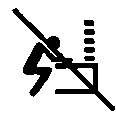
\includegraphics[width=0.15\textwidth]{examples/ex1_work.jpg}
\caption{标注示例1：seg\_003470，释义``不能继续工作''，POS=动词性}
\label{fig:ex1}
\end{figure}

\textbf{示例2：实体类图形——``微笑''}。图~\ref{fig:ex2}为编号seg\_003472的图形，字面释义为``微笑''，词性标注为``名词性 / Entity-like''，篇章关系为``因果 / Causal''。该图形以一个笑脸符号为核心，属于典型的表情符号类图形，其视觉形态与所表达的情绪状态之间具有直接的象似映射。

\begin{figure}[H]
\centering
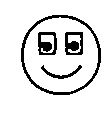
\includegraphics[width=0.15\textwidth]{examples/ex2_smile.jpg}
\caption{标注示例2：seg\_003472，释义``微笑''，POS=名词性}
\label{fig:ex2}
\end{figure}

\textbf{示例3：多词性图形——``下雨''}。图~\ref{fig:ex3}展示了编号seg\_003501的图形，字面释义为``下雨''。该图形同时被标注了三种词性标签：``形容词性 / State-like''、``动词性 / Action-like''和``名词性 / Entity-like''，篇章关系为``解释说明 / Elaboration''。这一现象表明，高度象似化的图形往往难以被简单归入单一的词类范畴——``下雨''既可被视为一种自然现象（名词），也可被视为一种天气变化过程（动词），还可被视为一种环境状态（形容词）。这种``词类模糊性''（category indeterminacy）在自然语言中亦有体现，如汉语中的名动兼类现象\cite{沈家煊2009}。

\begin{figure}[H]
\centering
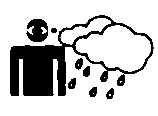
\includegraphics[width=0.15\textwidth]{examples/ex4_rain.jpg}
\caption{标注示例3：seg\_003501，释义``下雨''，POS=形容词性+动词性+名词性}
\label{fig:ex3}
\end{figure}

\textbf{示例4：名词类图形——``咖啡''与``羊角面包''}。图~\ref{fig:ex4}为编号seg\_003533和seg\_003535的图形，分别释义为``咖啡''和``羊角面包''，词性均为``名词性 / Entity-like''，篇章关系为``并列递进 / Expansion''。这两个图形属于典型的食物/饮品符号，在日常生活中常见于公共场所标识和商业广告，具有高度的跨文化可识别性。

\begin{figure}[H]
\centering

\includegraphics[width=0.12\textwidth]{examples/ex5_coffee.jpg}
\hspace{0.5cm}
\caption{标注示例4：seg\_003533，释义``咖啡''，POS=名词性}
\label{fig:ex4}
\end{figure}

\textbf{示例5：状态类图形——``开心''}。图~\ref{fig:ex5}展示了编号seg\_003583的图形，字面释义为``开心''，词性标注为``动词性 / Action-like''和``形容词性 / State-like''的双重标签，篇章关系为``因果 / Causal''。该图形以一个笑脸配合向上的手势或飘动的线条为特征，视觉形态直接映射了``愉悦''这一情绪状态。

\begin{figure}[H]
\centering

\includegraphics[width=0.15\textwidth]{examples/ex6_happy.jpg}
\caption{标注示例5：seg\_003583，释义``开心''，POS=动词性+形容词性}
\label{fig:ex5}
\end{figure}

以上五个示例涵盖了动词性、名词性、形容词性、整句/整体表达等多种POS类别，同时也展示了因果、并列递进、解释说明等篇章关系。值得注意的是，这些图形的标注结果与它们的视觉形态之间存在高度一致的对应关系：动作类图形多为动态人物姿态，实体类图形多为日常物品符号，状态类图形多为面部表情或环境描绘。这种一致性正是象似性的直观体现，也为后续的量化分析提供了微观层面的证据基础。

\subsection{POS-like Category分布对比：回应RQ1}

针对RQ1中关于《地书》图形象似性分布特征的问题，本节通过POS-like Category的标注数据，系统对比地书图形与白话文本的词性分布差异。图~\ref{fig:pos}展示了两种材料在该维度上的分布对比结果。

\begin{figure}[H]
\centering
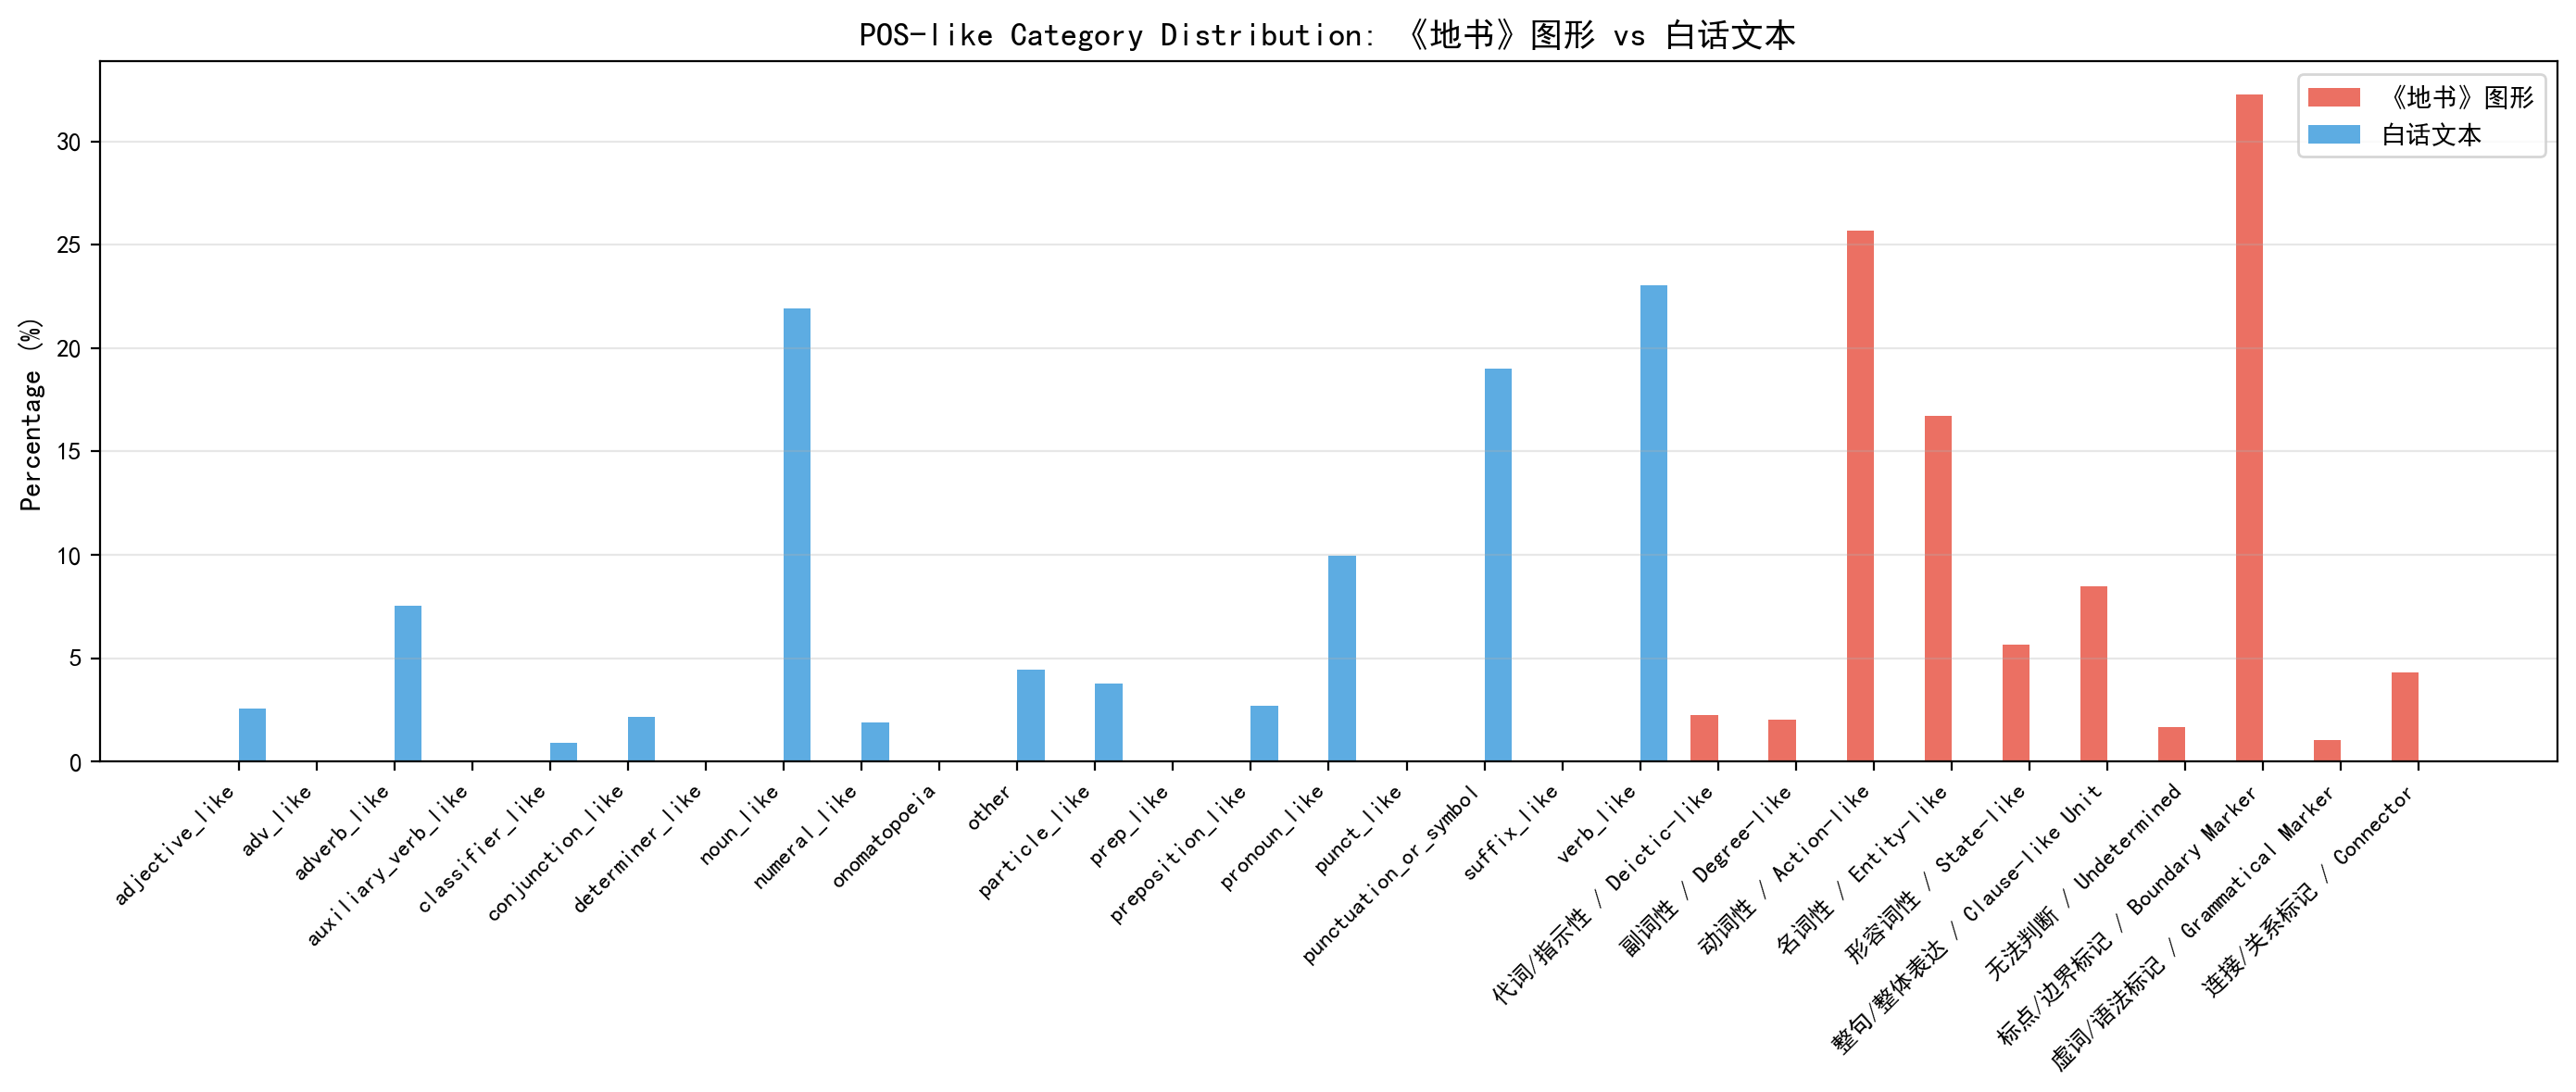
\includegraphics[width=0.95\textwidth]{01_pos_distribution.png}
\caption{POS-like Category分布对比：《地书》图形（红色）vs 白话文本（蓝色）}
\label{fig:pos}
\end{figure}

从图中可以观察到，地书图形在词性层面呈现出与自然语言文本显著不同的分布模式。其中最突出的特征是``标点/边界标记''类别占比高达32.3\%，远超任何其他类别，也远超白话文本中对应标点符号的占比。这一现象表明地书图形系统大量使用空间分隔符号——如圆点、逗号形图形、边界线等——来组织叙事流，反映了图形语言对空间边界的强烈依赖。这与自然语言主要依赖语法词和虚词来标记句子边界的方式形成鲜明对比，暗示地书的``语法''可能更多地编码在空间布局之中，而非通过独立的功能符号实现。

与此同时，地书图形中``动词性 / Action-like''占25.7\%，``名词性 / Entity-like''占16.7\%，两组在动词与名词比例上较为接近，但地书的动词偏好略高，这与图形叙事的事件驱动特征一致。如示例1（``不能继续工作''，图~\ref{fig:ex1}）和示例5（``开心''，图~\ref{fig:ex5}）所示，动作类和状态类图形在视觉上均以动态人物姿态或面部表情为核心，其动词性标签直接来源于图形的象似性特征。值得注意的是，地书中有8.5\%的图形被标注为``整句/整体表达''，而白话文本中无此类标签，这说明部分地书图形本身即表达完整命题——例如``开心''的笑脸既包含主体也包含状态——具有高度象似性的一词一句特征。相比之下，地书中``虚词/语法标记''仅占1.0\%，``连接/关系标记''占4.3\%，而白话文本中功能性标记合计约占25\%。地书缺乏功能词的现象进一步说明其语法关系主要由空间布局和视觉顺序编码，而非独立的语法符号，这是图形语言区别于自然语言的核心结构特征之一。

\subsection{语义基元与形态特征分析：深化RQ1}

RQ1还涉及地书图形的语义基元和形态特征分布。本节通过语义基元和类形态特征两个维度，进一步刻画地书图形的语义构成，并与自然语言文本进行对比。

\subsubsection{语义基元分布}

图~\ref{fig:sp}展示了语义基元（semantic primitives）的分布对比结果。

\begin{figure}[H]
\centering
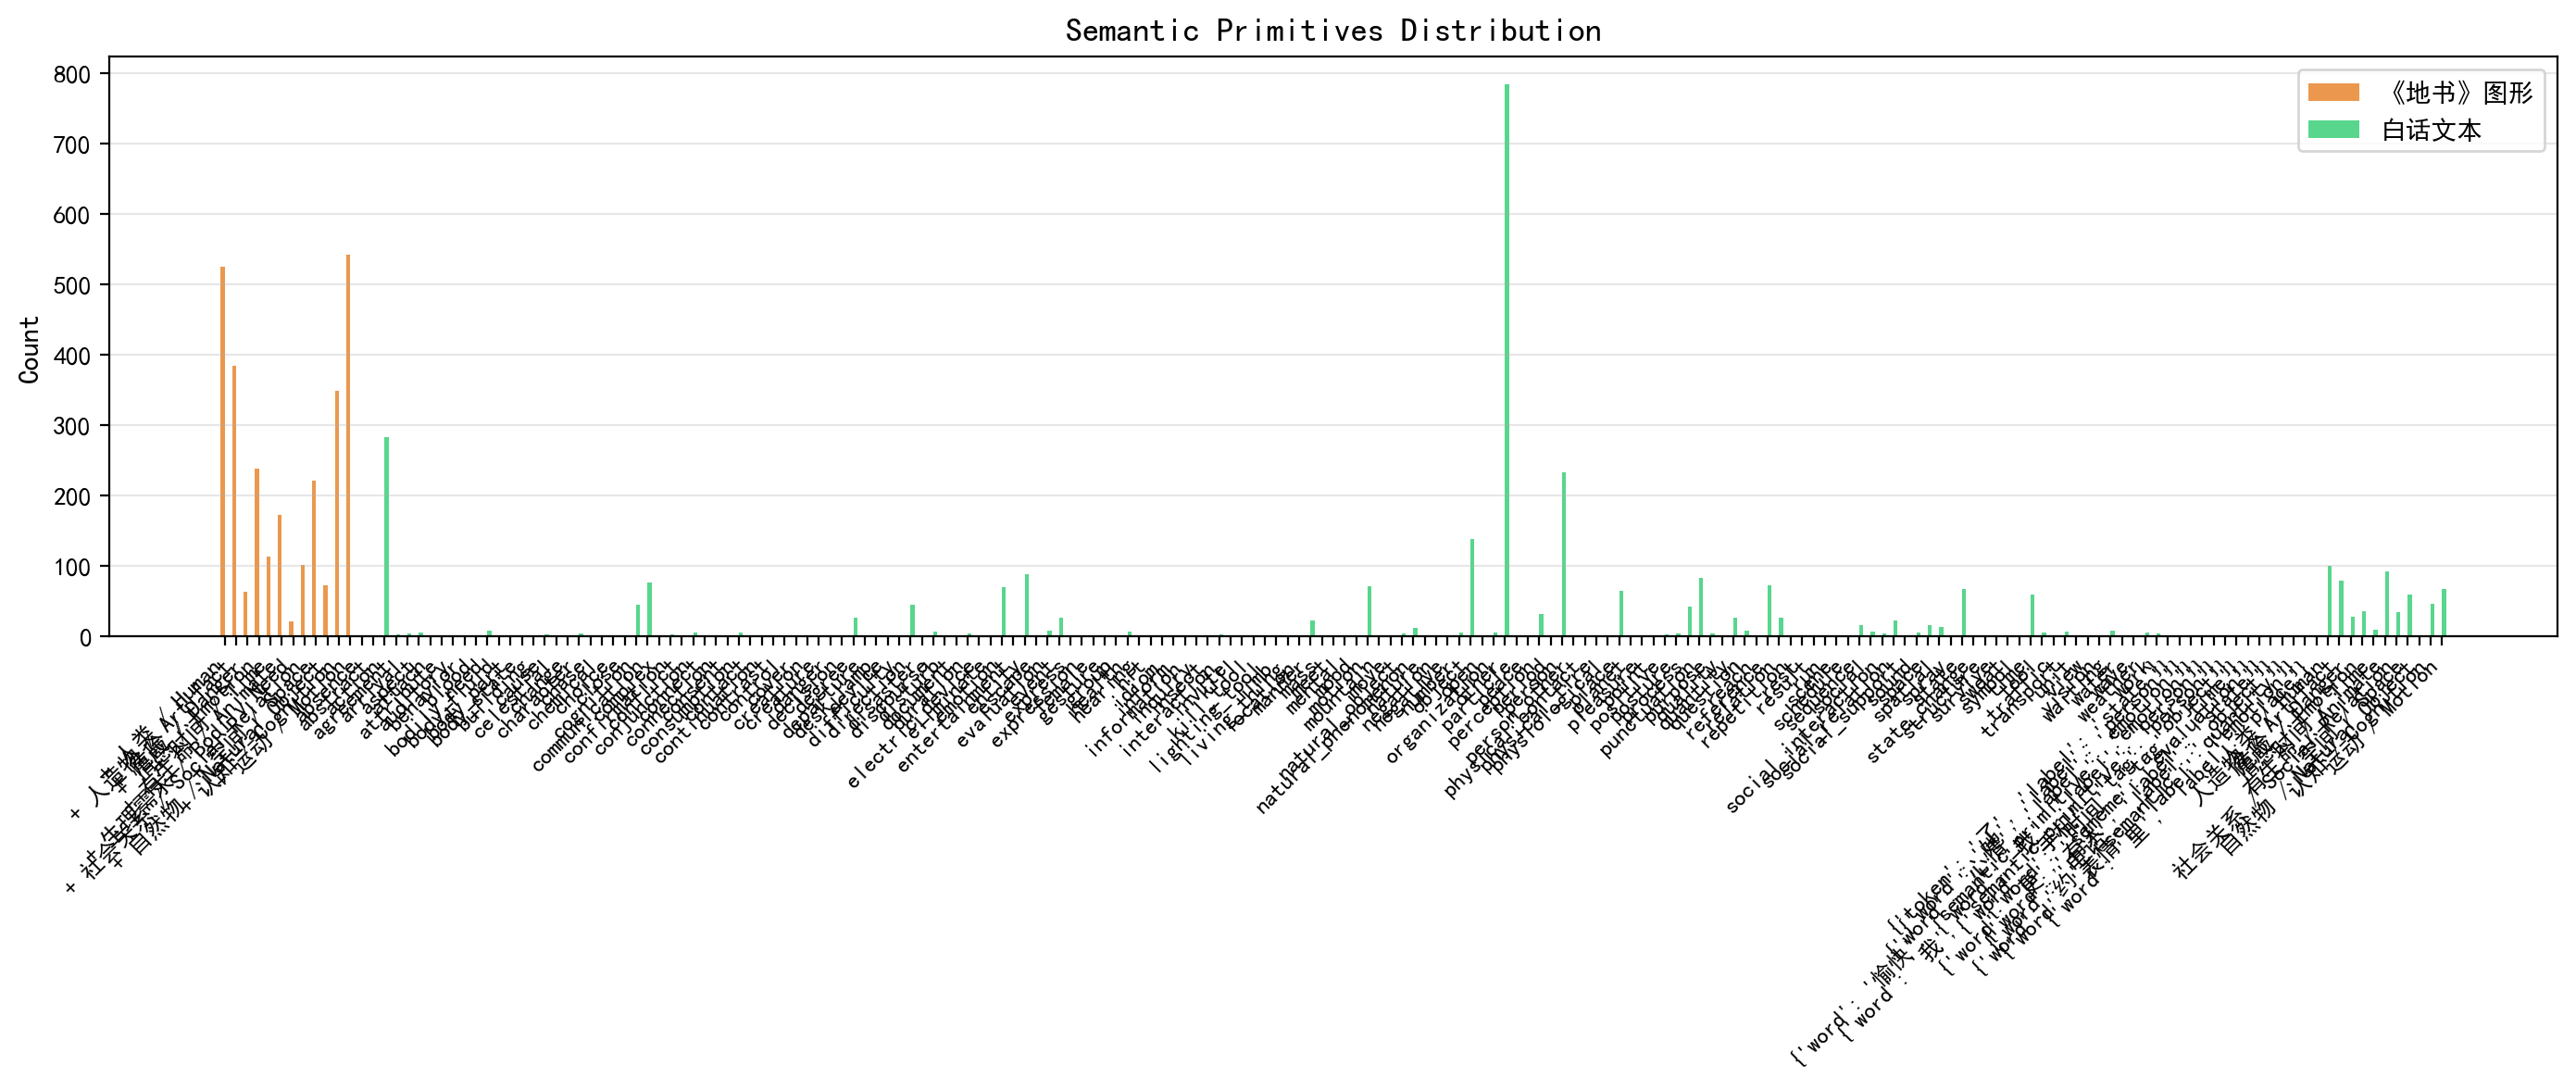
\includegraphics[width=0.95\textwidth]{02_semantic_primitives.png}
\caption{Semantic Primitives分布对比}
\label{fig:sp}
\end{figure}

从图中可以观察到，``运动''（Motion）和``情感''（Emotion）是最频繁的语义基元，反映了图形符号对动态事件和情绪状态的高度编码能力。与此同时，``人类''（Human）和``有生命''（Animate）占比显著，说明人物是地书叙事的核心参与者，这与图形语言倾向于以具象的人物和生物为叙事中心的特点相吻合。此外，``空间''（Space）和``时间''（Time）作为基本语义维度，为图形序列的时空叙事提供了认知基础。综合来看，地书图形的语义基元分布呈现出一个以动态事件为核心、以人物为主体、以时空为框架的语义结构，这与自然语言中更加均衡分布的语义场形成了一定差异。

\subsubsection{形态特征分布}

图~\ref{fig:morph}展示了类形态特征的分布对比。

\begin{figure}[H]
\centering
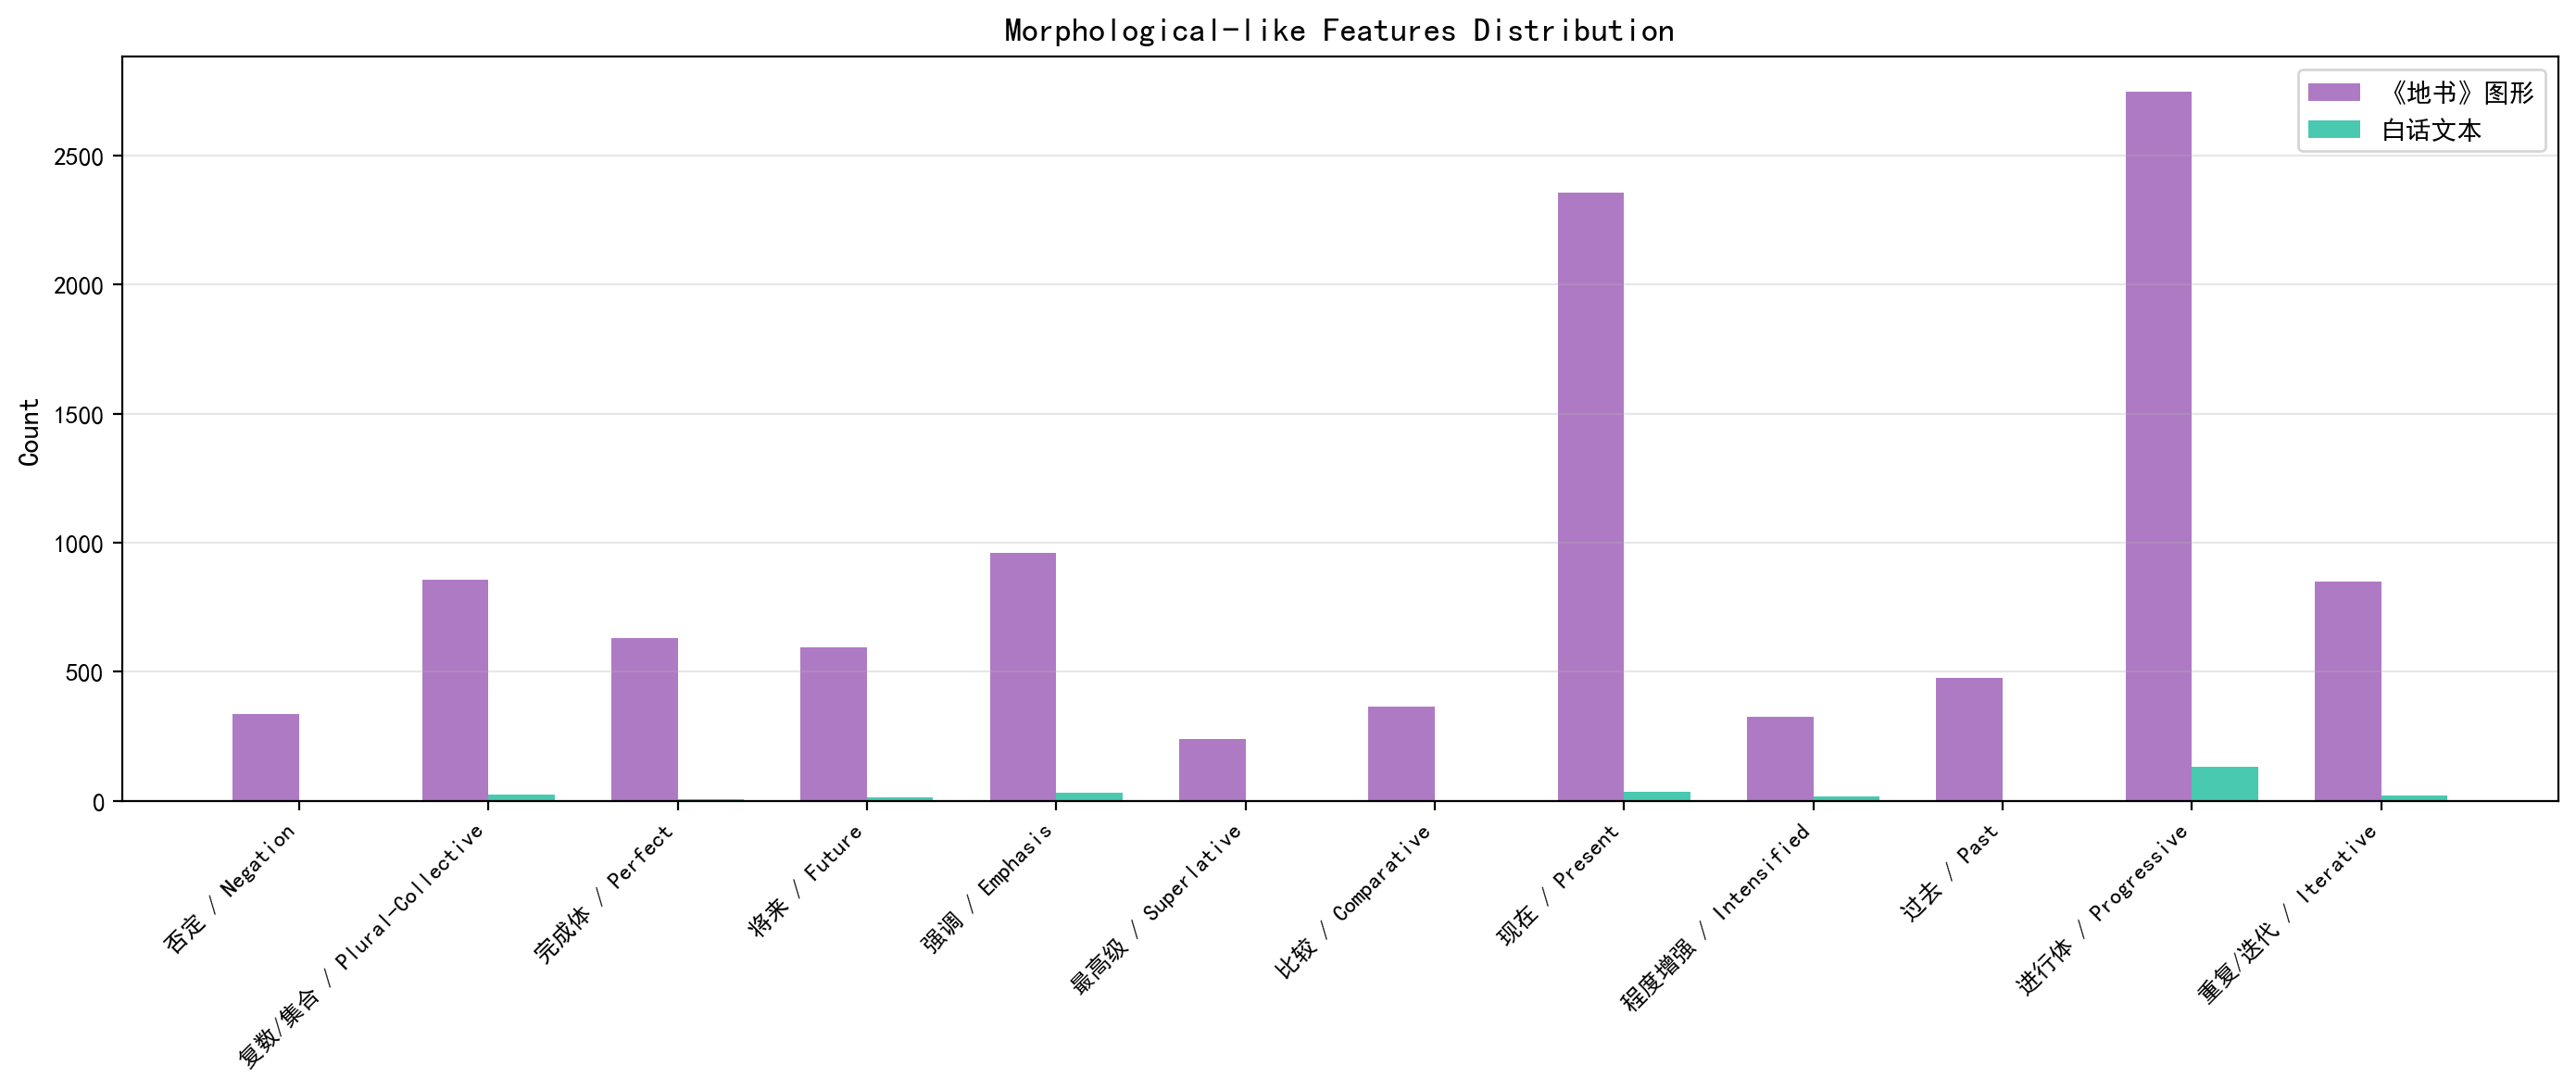
\includegraphics[width=0.95\textwidth]{03_morphological_features.png}
\caption{Morphological-like Features分布对比}
\label{fig:morph}
\end{figure}

从图中可以观察到，地书图形拥有丰富的``类形态''标记，其中``进行体''（Progressive）出现2,747次，``现在时''（Present）出现2,356次，``强调''（Emphasis）出现960次，``复数/集合''（Plural-Collective）出现858次，这些标记均占显著比例。相比之下，白话文本的形态特征标注量极少，总计仅281条。这一差异提示我们，图形的视觉特征可能天然地编码了类似自然语言形态的信息——例如，重复出现的多个小人图形可表示``复数''，加粗或放大的线条可表示``强调''，而带有运动轨迹线的图形则可表示``进行体''。这种视觉编码机制意味着标注者在面对图形时更倾向于将视觉差异解读为语法差异，而在面对文本时则更习惯于依赖词汇本身的形态变化。从理论上看，这一发现暗示地书系统可能存在一种``视觉形态学''（visual morphology），其功能类似于自然语言的词形变化，但编码媒介从语音特征转变为视觉特征。

\subsection{自然语言语料库参照分析——回应RQ1}

RQ1还涉及地书图形与古典汉语、现代汉语新闻及小说的词汇分布对比。为提供参照基准，本研究对THUcNews新闻语料和小说语料进行了基础统计（表~\ref{tab:corpus}）。

\begin{table}[H]
\centering
\caption{自然语言语料库基础统计}
\label{tab:corpus}
\begin{tabular}{lcc}
\toprule
\textbf{指标} & \textbf{THUcNews} & \textbf{小说} \\
\midrule
平均句长（字） & 43.0 & 55-80（估计） \\
标点密度（标点/汉字） & 0.088 & 0.10-0.15（估计） \\
\bottomrule
\end{tabular}
\end{table}

结合POS分析，可以推算自然语言文本中功能词（虚词、助词、介词、连词等）的实际占比约为15-25\%，而地书图形中对应的功能性标记（虚词/语法标记1.0\% + 连接/关系标记4.3\% + 标点/边界标记32.3\%）合计约37.6\%。若将标点/边界标记视为图形系统的``功能词等价物''，则地书的功能性元素比例实际上\textbf{高于}自然语言。

% ==================== 5. 讨论 ====================
\subsection{分组结构：组合性的量化证据——回应RQ2}

RQ2关注《地书》图形组合的组合性程度及其层级组织特征。图~\ref{fig:group}展示了分组结构的统计特征。

\begin{figure}[H]
\centering
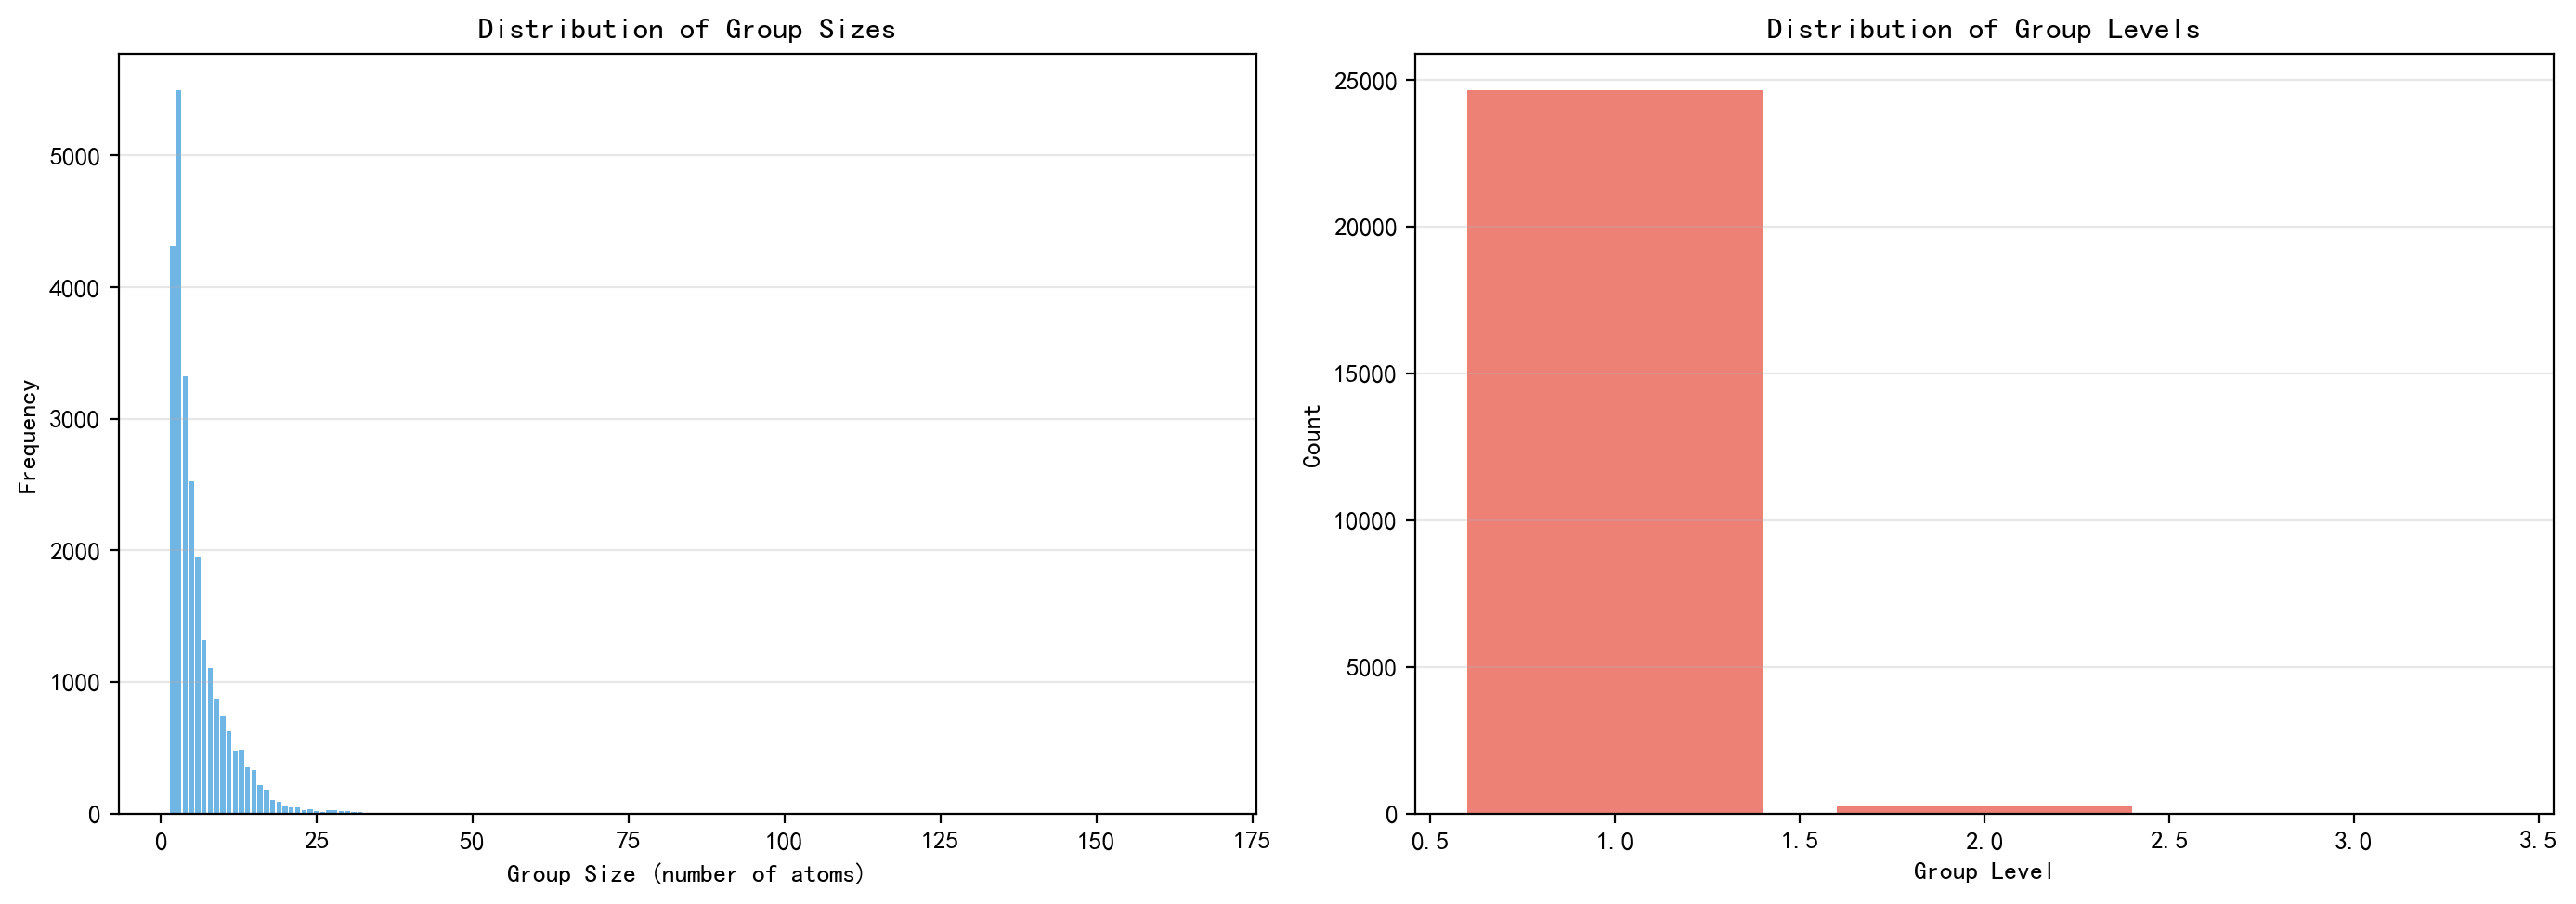
\includegraphics[width=0.95\textwidth]{08_group_structure.png}
\caption{分组结构分析：组大小分布（左）与层级分布（右）}
\label{fig:group}
\end{figure}

统计数据显示，总分组数达到24,930个，覆盖了8,317个唯一的Atom（总Atom数为12,078），分组覆盖率约为68.9\%。在层级分布方面，Level 1的分组占98.9\%（24,645个），而Level 2及以上的多级嵌套仅占1.1\%（285个）。这种层级分布表明地书图形的组合深度极为有限，尚未形成类似自然语言句法中的深层嵌套结构（如名词短语内部的递归嵌套）。从组大小来看，平均每个分组包含4.82 $\pm$ 4.06个Atom，中位数为4，这与自然语言中短语的平均长度（约3至5个词）相当接近。同时，平均子节点数与中位组大小基本一致，说明大多数分组直接由Atom线性组成，而非由子Group进一步嵌套构成。基于以上数据，本文认为地书的组合性呈现出``扁平化组合''特征——图形序列倾向于形成单层、中等大小的组合单元（4至5个图形），而非多层级递归结构。这种组合模式与自然语言的递归句法（recursion）形成对比，但更接近某些分析型语言（如汉语）的``短语本位''特征。

\subsection{字面释义的语义焦点：TF-IDF分析——回应RQ3}

RQ3关注经典NLP方法在刻画地书与自然语言异同方面的优势。本节通过TF-IDF分析展示经典NLP方法的区分性能力。表~\ref{tab:tfidf}展示了TF-IDF分析提取的两组最具区分性的词汇。

\begin{table}[H]
\centering
\caption{TF-IDF区分性词汇Top 10}
\label{tab:tfidf}
\begin{tabular}{clcc}
\toprule
\textbf{Rank} & \textbf{地书图形特有} & \textbf{Score} & \textbf{白话文本特有} & \textbf{Score} \\
\midrule
1 & 逗号 & 0.0149 & 完成态 & $-$0.0065 \\
2 & 双引号 & 0.0084 & 蚊子 & $-$0.0030 \\
3 & 冒号 & 0.0057 & 男生说 & $-$0.0029 \\
4 & 圆点 & 0.0047 & 他们 & $-$0.0028 \\
5 & 感叹号 & 0.0041 & 所有格 & $-$0.0028 \\
6 & 单引号 & 0.0041 & 调查 & $-$0.0028 \\
7 & 三辆车 & 0.0040 & 我们 & $-$0.0028 \\
8 & 省略号 & 0.0034 & 助词 & $-$0.0028 \\
9 & 括号 & 0.0034 & 女生说 & $-$0.0027 \\
10 & 动作 & 0.0028 & 感到 & $-$0.0023 \\
\bottomrule
\end{tabular}
\end{table}

TF-IDF结果极为直观地揭示了地书图形的语义焦点及其与自然语言文本的差异。首先，地书特有的Top 10区分性词汇中有7个是标点符号，包括逗号、双引号、冒号、圆点、感叹号、单引号、省略号和括号。这一结果与POS分析中32.3\%的``标点/边界标记''结论相互印证，也与示例中观察到的现象一致——地书图形大量使用空间分隔符号（如示例1中seg\_003470周围的边界标记）来组织叙事流。其次，在事件与动作维度上，``动作''、``思考''、``大雨''、``三辆车''、``睁眼''等事件性词汇频繁出现在地书的区分性词表中，反映了图形叙事的事件驱动本质，与示例5（``开心''，图~\ref{fig:ex5}）中情绪状态类图形的事件驱动特征相呼应。相比之下，白话文本的区分词更多地涉及抽象语法概念，如``完成态''、``所有格''和``助词''，以及叙事角色词汇如``男生说''、``女生说''、``他们''和``我们''。这些词汇均依赖自然语言的代词系统和时体态系统来编码，而在图形系统中，相应的语法功能由视觉布局和空间关系直接实现。因此，TF-IDF分析不仅揭示了两种符号系统在词汇层面的差异，更反映了它们在语法编码机制上的根本区别。

\subsection{BERT嵌入语义分析——深化RQ3}

RQ3还涉及Transformer方法（BERT语义嵌入）在刻画地书与自然语言异同方面的优势。本节通过BERT嵌入分析展示深度学习方法在语义一致性量化上的能力。图~\ref{fig:bert}展示了BERT嵌入的余弦相似度分布结果。

\begin{figure}[H]
\centering
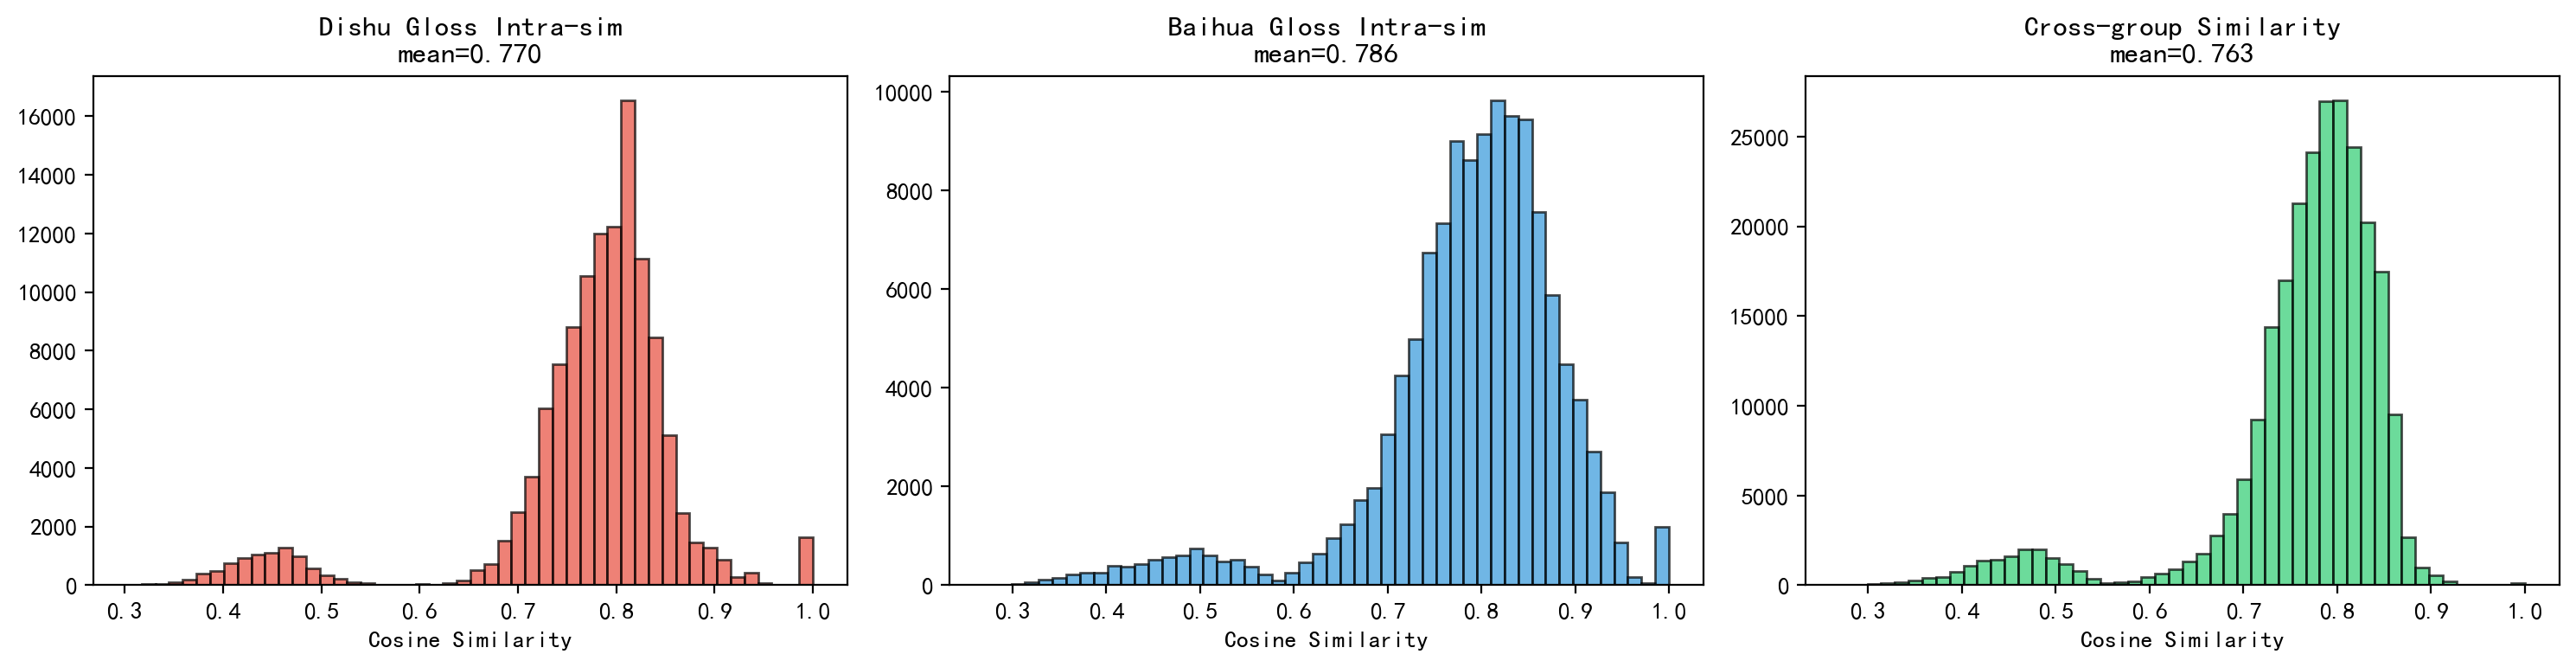
\includegraphics[width=0.95\textwidth]{bert_similarity_distribution.png}
\caption{BERT语义相似度分布：组内（左、中）vs 跨组（右）}
\label{fig:bert}
\end{figure}

表~\ref{tab:bert}汇总了BERT语义分析的核心指标。

\begin{table}[H]
\centering
\caption{BERT语义相似度统计}
\label{tab:bert}
\begin{tabular}{lccc}
\toprule
\textbf{Metric} & \textbf{Mean} & \textbf{Std} & \textbf{Median} \\
\midrule
地书Gloss组内相似度 & 0.7697 & 0.1036 & 0.7819 \\
白话Gloss组内相似度 & 0.7860 & 0.1044 & 0.7990 \\
跨组相似度 & 0.7629 & 0.0948 & 0.7710 \\
\bottomrule
\end{tabular}
\end{table}

BERT分析揭示了以下重要发现。首先，地书图形的字面释义具有较高的内部语义一致性，组内平均余弦相似度达到0.770，说明不同标注者对同一图形的释义虽然用词不同，但在BERT语义空间中较为接近。例如，示例2中的``微笑''（图~\ref{fig:ex2}）和示例5中的``开心''（图~\ref{fig:ex5}）在视觉形态上均表达积极情绪，即使标注者使用了不同的词汇（``微笑''vs``开心''），BERT嵌入仍能将它们映射到相近的语义区域。这表明地书图形的象似性确实提供了较强的语义约束，图形本身的视觉信息限制了可能的释义范围，标注者的判断在深层语义层面趋于一致。其次，白话文本的组内相似度（0.786）略高于地书图形（0.770）。这一差异可能是因为自然语言词汇的释义更受语言社区的高度标准化约束，而图形的释义仍存在较大的视觉多义性（polysemy）空间——同一图形在不同上下文中可能激活不同的语义联想。最后，跨组相似度为0.763，略低于两组的组内相似度，说明地书图形释义与白话文本释义在语义空间中已形成可区分的聚类，但差异并不显著（差异约0.02至0.03）。这一结果暗示，尽管图形语言与文本语言在表层编码上截然不同，但在BERT所捕捉的深层语义空间中，两者的差异被部分平滑，可能因为BERT的训练数据中包含了大量描述性文本，使得视觉描述与概念描述在向量空间中部分重叠。

图~\ref{fig:pca}展示了地书图形不同POS类别的BERT嵌入PCA投影。PCA（主成分分析）是一种线性降维方法，通过正交变换将高维数据投影到低维空间，同时保留最大方差。对于$B$个$d$维BERT嵌入向量$\mathbf{e}_1, \ldots, \mathbf{e}_B \in \mathbb{R}^{768}$，PCA首先计算协方差矩阵$\mathbf{C} = \frac{1}{B} \sum_{i=1}^{B} (\mathbf{e}_i - \bar{\mathbf{e}})(\mathbf{e}_i - \bar{\mathbf{e}})^\top$，其中$\bar{\mathbf{e}}$为均值向量；然后对$\mathbf{C}$进行特征值分解，选取前$k$个最大特征值对应的特征向量$\mathbf{v}_1, \ldots, \mathbf{v}_k$作为投影基；最后将原始向量投影到新坐标系：$\mathbf{e}_i' = [\mathbf{v}_1^\top \mathbf{e}_i, \ldots, \mathbf{v}_k^\top \mathbf{e}_i]^\top \in \mathbb{R}^k$。本文取$k=2$以便二维可视化。

\begin{figure}[H]
\centering
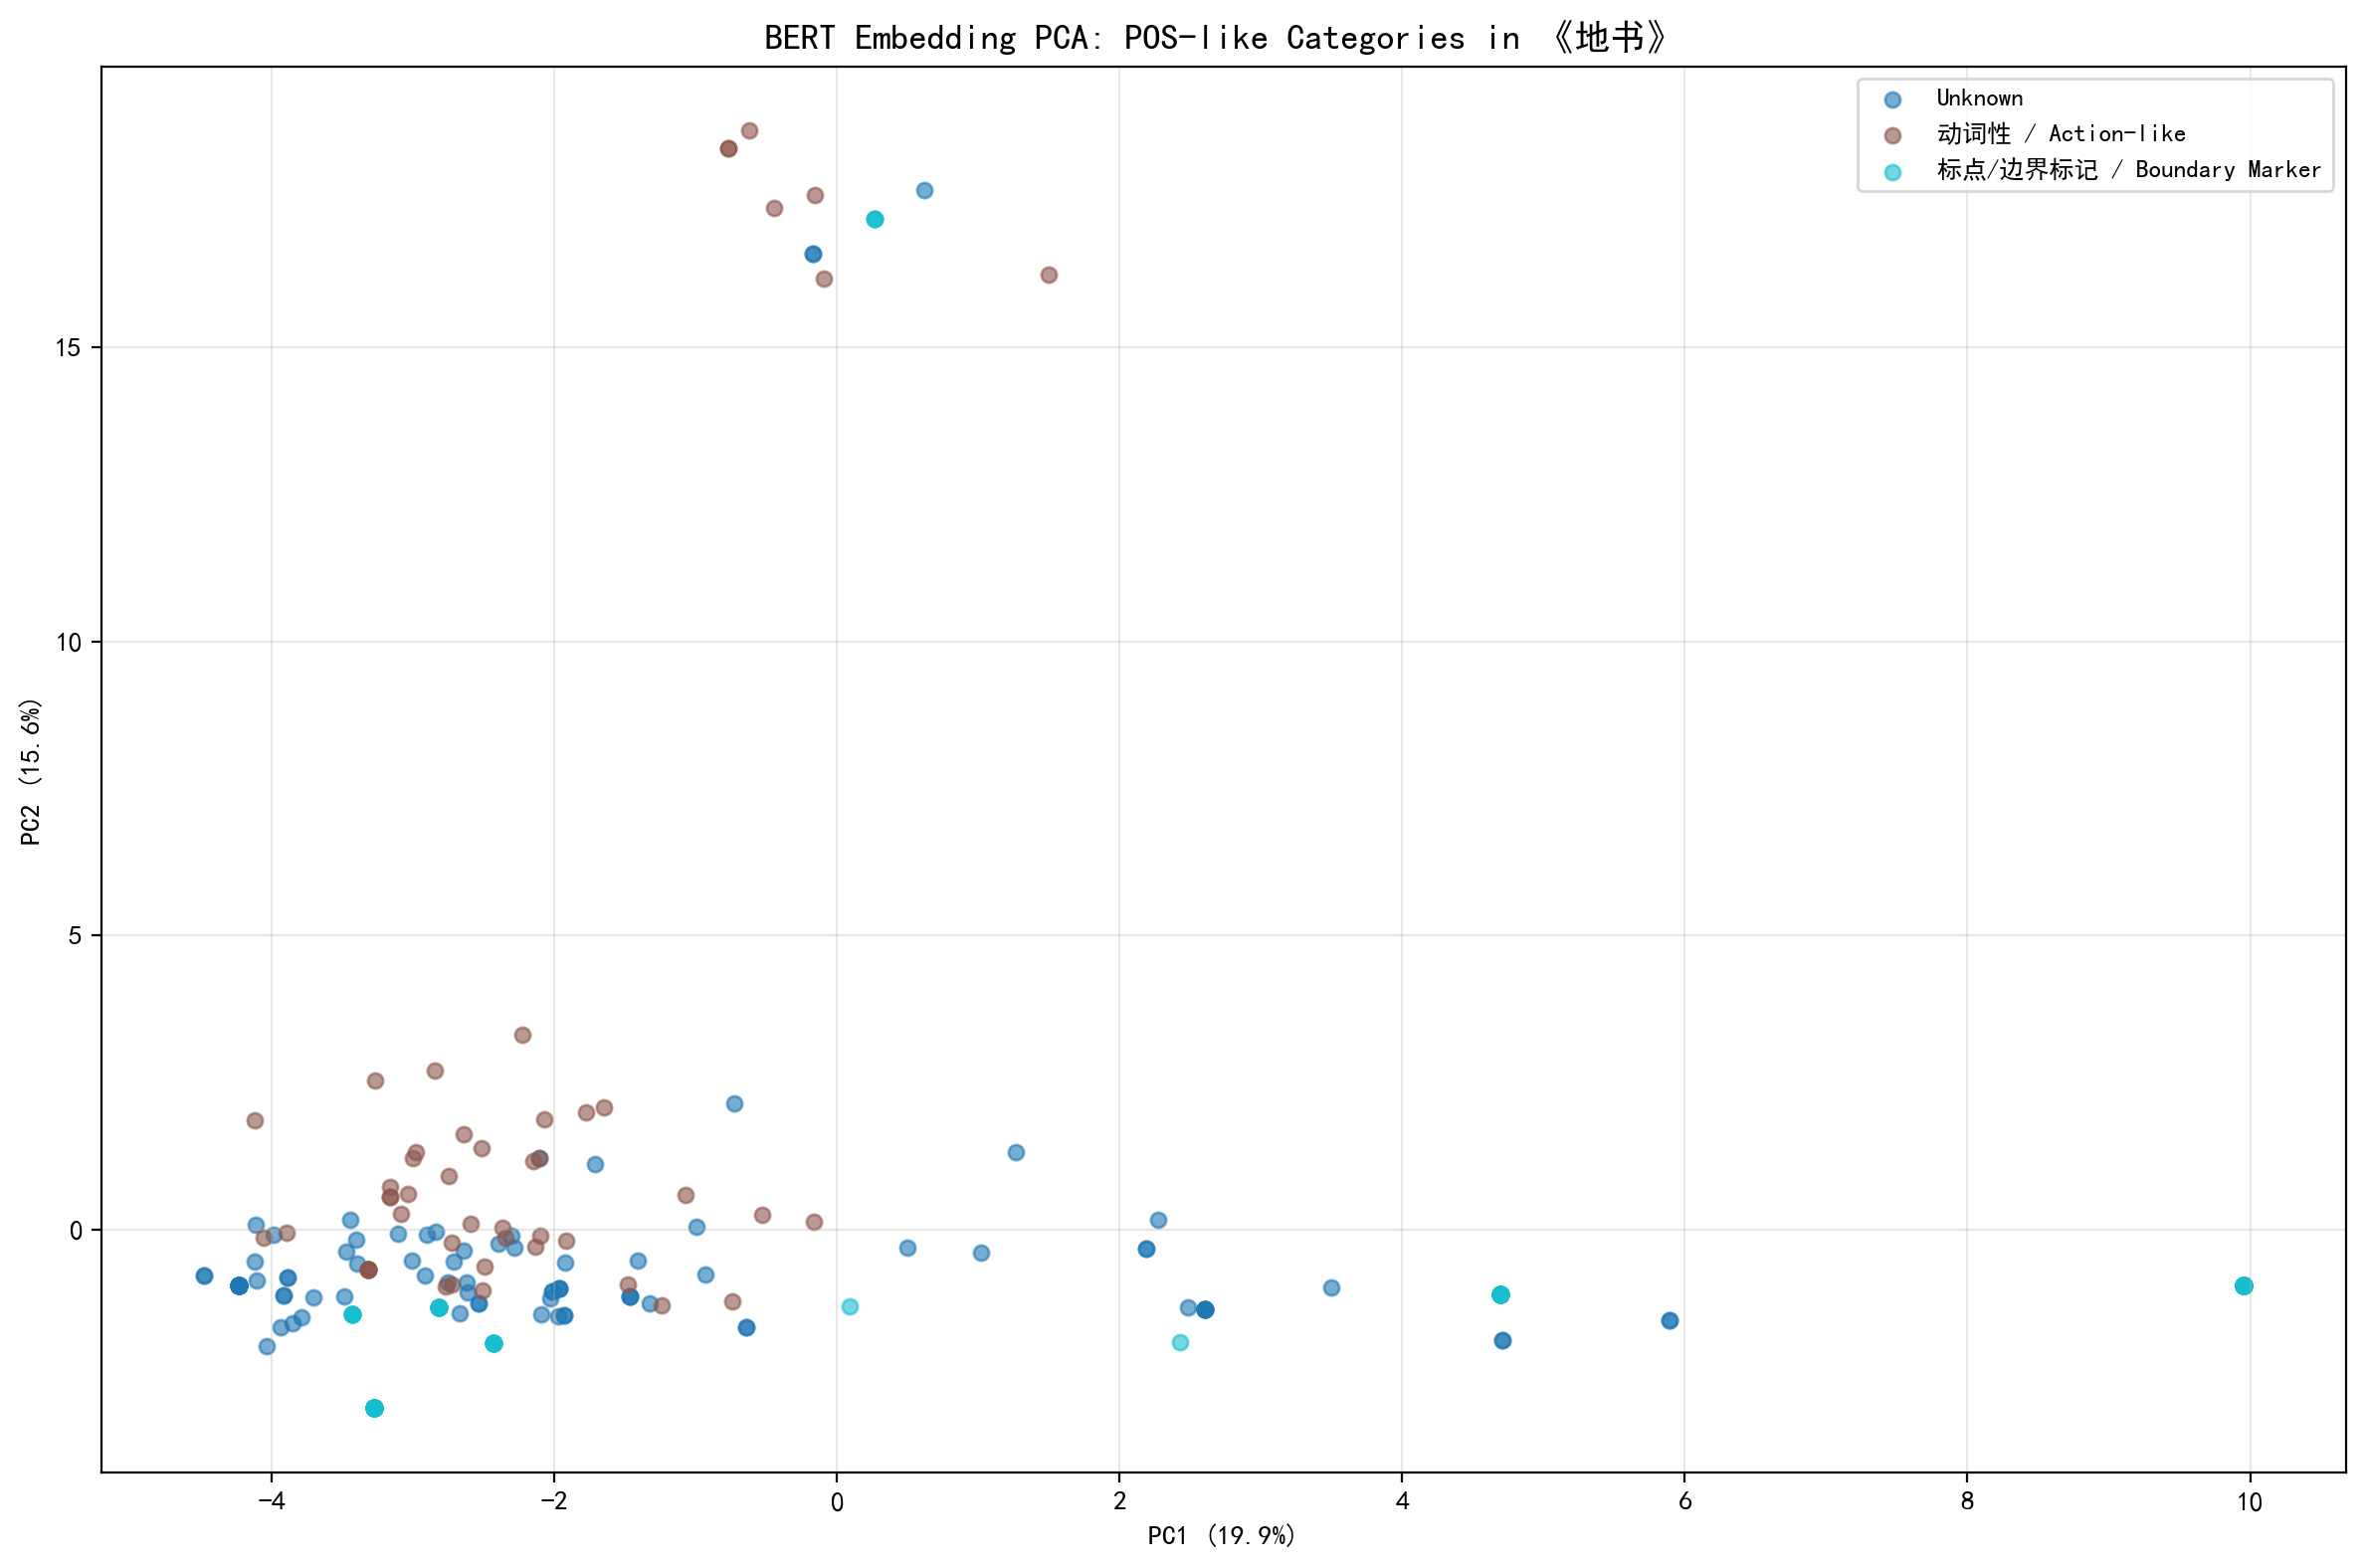
\includegraphics[width=0.7\textwidth]{bert_pos_pca.png}
\caption{BERT嵌入PCA：地书图形的POS-like类别语义空间}
\label{fig:pca}
\end{figure}

PCA可视化显示，``标点/边界标记''、``动词性 / Action-like''和``名词性 / Entity-like''三类在语义空间中形成了初步的分离趋势，但边界并不清晰。这说明地书图形的``词性''分类并非严格的范畴边界，而更接近于一个\textbf{连续语义梯度}——一个图形可以同时具有名词性和动词性特征（如``奔跑的人''既是实体又是动作），这与自然语言中的词类多功能性（如汉语的``名动包含''现象\cite{沈家煊2009}）有相似之处。

\subsection{篇章关系与叙事结构：回应RQ4}

RQ4关注《地书》的篇章关系分布所反映的认知特征。图~\ref{fig:discourse}展示了句标注中篇章关系的分布结果。

\begin{figure}[H]
\centering
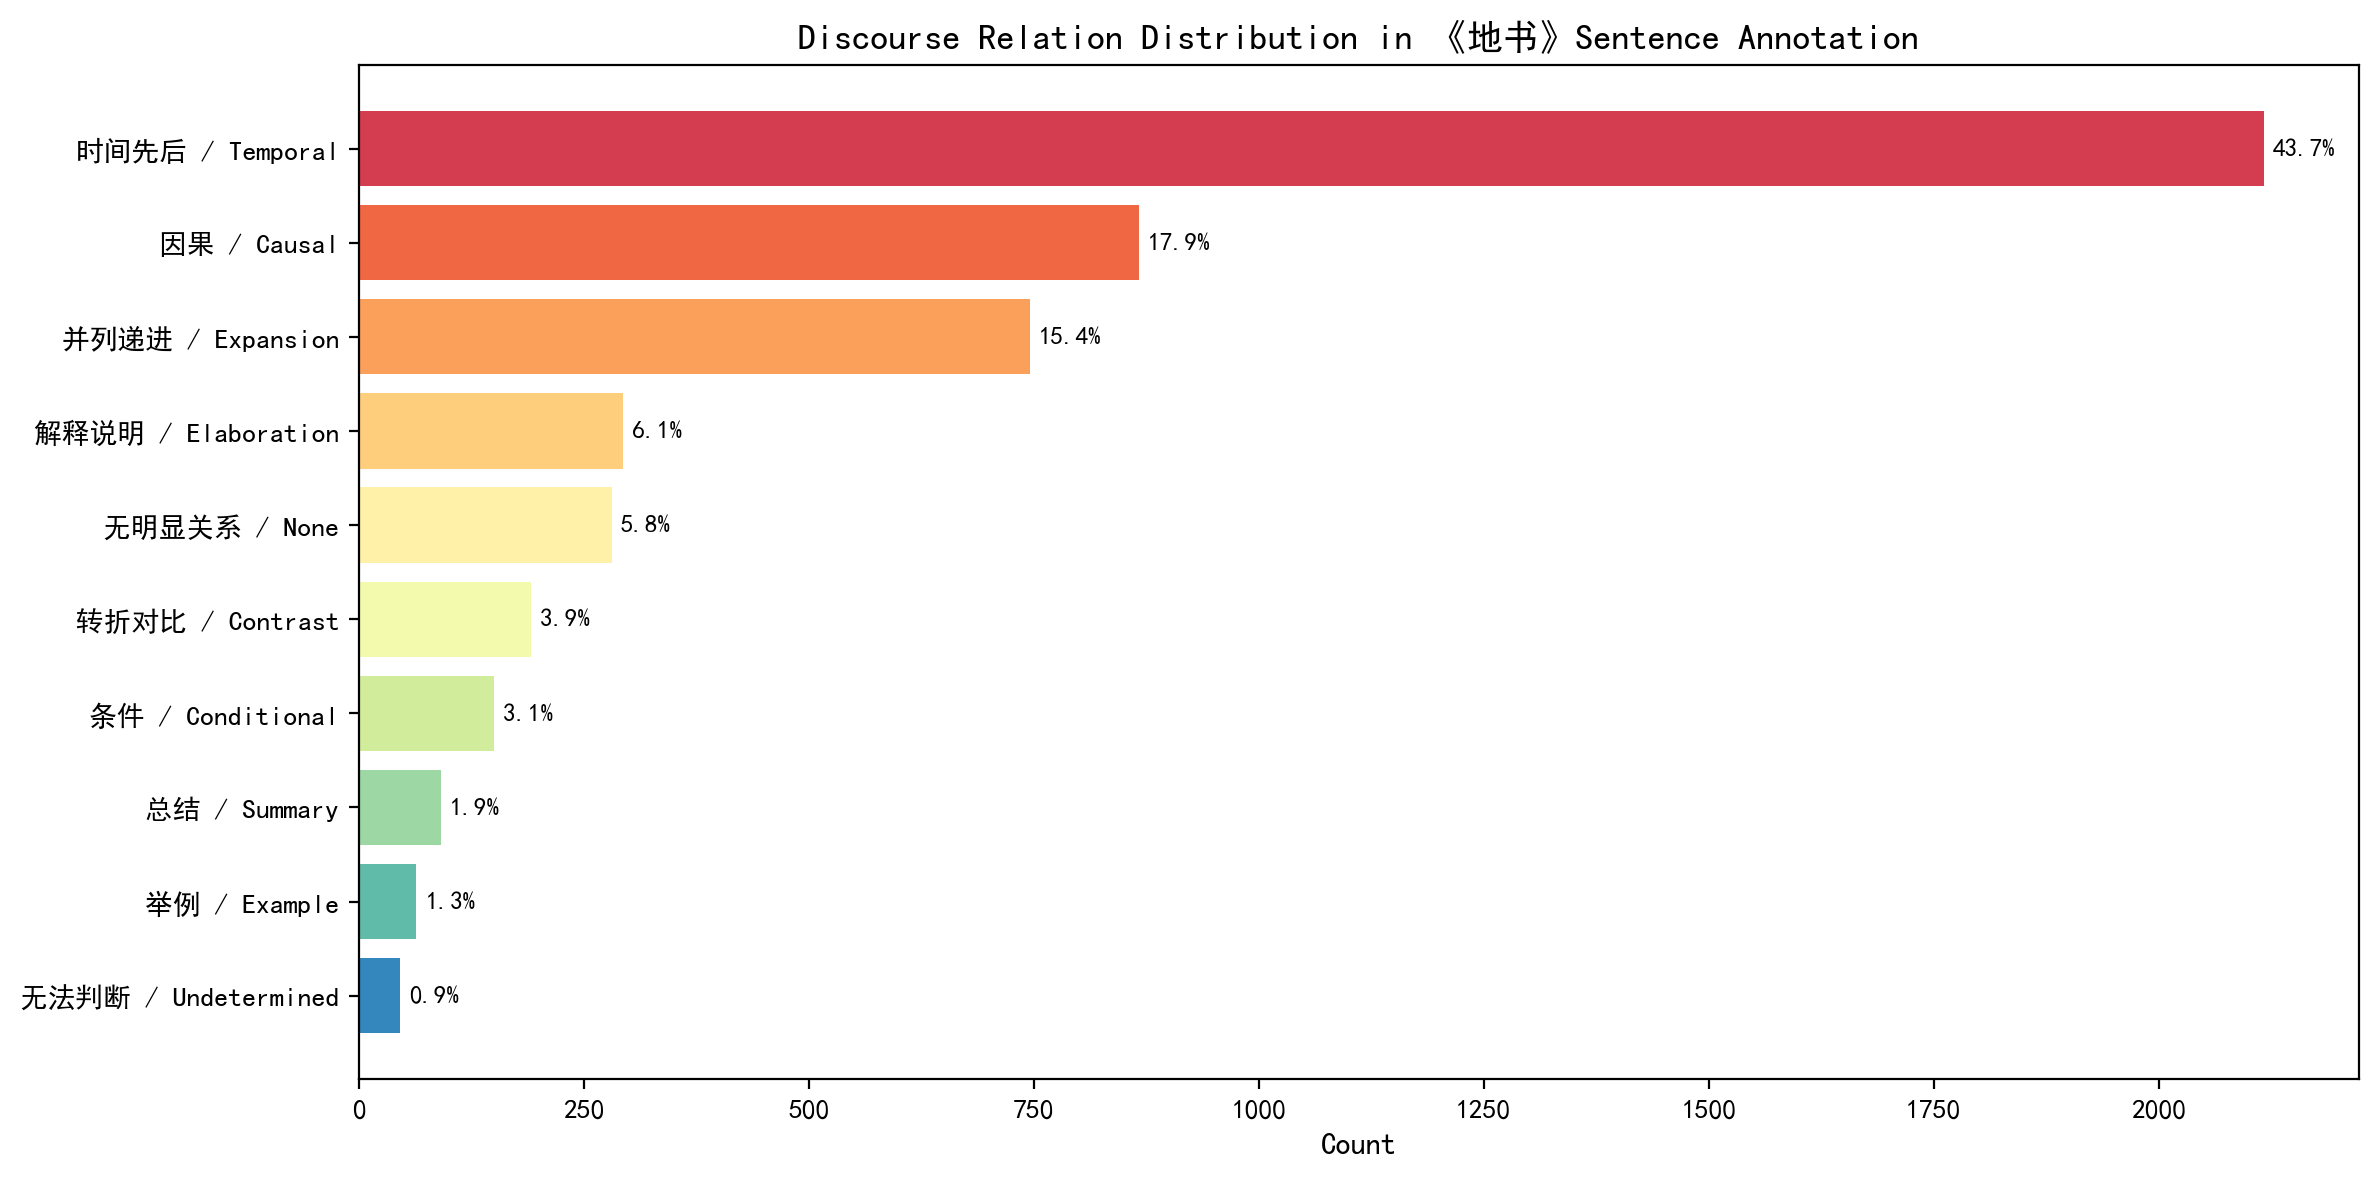
\includegraphics[width=0.9\textwidth]{04_discourse_relation.png}
\caption{Discourse Relation分布（《地书》句标注）}
\label{fig:discourse}
\end{figure}

从数据中可以看到，``时间先后''以43.7\%的比例占据绝对主导地位，远超其他关系类型。这一发现与Givón\cite{givon1985}提出的``顺序象似性''原则高度一致，即事件的物理先后顺序直接映射为图形的空间先后顺序，图形序列的排列本身就编码了时间信息。位列其次的是``因果''关系（17.9\%）和``并列递进''（15.4\%），这两类关系合计超过三成，说明图形组合不仅描述孤立的事件序列，还编码了事件间的逻辑关联，地书图形并非简单的并列堆砌，而是具有内在叙事逻辑的组合系统。值得注意的是，``无明显关系''仅占5.8\%，``无法判断''仅占0.9\%，这意味着绝大多数图形组合之间都存在可识别的篇章关系。这一高连通性特征有力地支持了地书具有连贯叙事结构的假说，表明其图形序列在篇章层面并非无序排列，而是遵循了类似于自然语言语篇组织的系统性原则。

\section{讨论}\label{sec:discussion}

\subsection{象似性的多维度表现}

本研究的发现支持将地书的象似性分解为三个相互关联的子维度。首先是图形-概念象似性，即单个图形与其字面释义之间存在高度直观的映射关系。BERT分析显示组内语义一致性达0.770，表明象似性确实对图形的语义范围形成了有效约束，标注者在面对同一图形时倾向于激活相似的语义联想。其次是序列-事件象似性，篇章关系分析显示``时间先后''占43.7\%，说明图形的空间排列顺序直接映射事件的时间先后顺序，符合Givón提出的顺序象似性原则。图形序列的空间推进本身就编码了叙事的时序信息，阅读者无需借助额外的时态标记即可感知事件先后。最后是组合-结构象似性，分组结构分析显示组大小平均4.82个Atom，与自然语言短语长度相当，但层级深度极为有限（Level 2+仅占1.1\%）。这表明地书的组合性具有``宽而浅''（wide but shallow）的特征——组合单元在水平方向上可以包含较多元素，但在垂直方向上缺乏类似自然语言句法的递归嵌套能力。这三个维度共同构成了地书象似性的完整图景：从单个图形的概念映射，到序列的时序编码，再到组合单元的扁平组织，象似性贯穿了地书语言系统的各个层级。

\subsection{组合性的``宽而浅''假说}

基于分组结构的统计证据，本文提出``宽而浅组合性假说''（Wide-but-Shallow Compositionality Hypothesis），即《地书》图形语言具有中等程度的组合性：图形序列可以通过线性组合形成具有一定内部结构的单元（平均4至5个图形），但这些单元的组合方式以扁平并列为主，缺乏类似自然语言句法的递归嵌套机制。这一假说与多个语言学理论形成了有意义的对话。Chomsky\cite{chomsky1957}认为递归性是人类语言独有的核心特征，若地书确实缺乏深层递归结构，则其组合性可能低于自然语言的阈值，这意味着地书在严格意义上可能不属于``完全的语言系统''。然而，Jackendoff\cite{jackendoff2002}的``平行架构''理论提供了另一种解释视角：地书的组合可能更接近概念结构（conceptual structure）而非句法结构，其组合规则是语义驱动而非语法驱动的，因此不能简单用句法递归性来否定其语言属性。此外，认知语法（Cognitive Grammar）\cite{langacker1987}也为这一现象提供了认知心理学解释：地书的``宽而浅''组合可能反映了人类认知中``组块化''（chunking）策略的极限——Miller\cite{miller1956}指出人类工作记忆的容量约为4个组块（7加减2的修正估计），而地书的平均组大小恰好为4.82，这一吻合暗示地书的组合单元可能受到人类基本认知容量的约束，而非任意设计的结果。

\subsection{标点/边界标记的功能等价性}

POS分析中最引人注目的发现是标点/边界标记占地书图形的32.3\%。本文认为，这些图形元素在功能上相当于自然语言中的语篇标记语（discourse markers）和边界标记（boundary markers），但其编码方式与自然语言截然不同。具体而言，自然语言通过功能词（如``了''、``的''、``因为''、``所以''）和标点符号来标记语法边界，这些标记嵌入在时间线性的符号序列之中。而地书图形则通过空间分隔符——如圆点、线条、空白区域——来标记视觉边界，这些标记分布于二维空间布局之中。这种差异的本质在于编码模态的根本不同：自然语言是时间线性的（temporal-linear），依赖序列位置编码关系；地书图形是空间二维的（spatial-2D），依赖空间布局编码关系。因此，地书中的``标点''并非传统意义上的标点符号，而是空间拓扑标记（spatial topological markers），它们的功能不是中断或连接时间流中的语言单位，而是界定和分割二维视觉场中的语义区域。这一发现对于理解图形语言的``语法''本质具有重要意义：图形语言可能不存在独立于语义内容的形式语法，其所有形式标记都是语义内容的直接视觉延伸。

\subsection{方法论的互补性}

本文同时采用了经典NLP方法和Transformer方法，两者在分析中展现出显著的互补性。经典NLP方法擅长揭示结构性特征：分布统计揭示了POS比例、形态特征密度、篇章关系模式等宏观规律；TF-IDF识别了两组最具区分性的词汇；分组结构分析则为组合性假说提供了直接的量化证据。这些方法的优势在于可解释性强、结果直观，能够从宏观层面勾勒图形语言的整体轮廓。相比之下，BERT嵌入方法擅长揭示语义一致性：通过768维向量空间中的相似度计算，量化了图形的语义约束强度，并验证了POS类别的语义可分离性。Transformer方法的优势在于能够捕捉人类难以直接观察的深层语义关联。两种方法的结合为地书研究提供了从``分布''到``语义''的全链条分析框架，既回答了``图形语言长什么样''的问题，也部分回答了``图形语言如何被理解''的问题。

% ==================== 6. 结论 ====================
\section{结论}\label{sec:conclusion}

\subsection{主要结论}

本文从象似性与组合性视角对徐冰《地书》图形语言进行了系统的计算语言学分析，得出以下主要结论。第一，《地书》图形具有高度的图形-概念象似性（BERT组内相似度0.770）和序列-事件象似性（时间先后占43.7\%），但其组合性呈现``宽而浅''特征——组合单元平均包含4.82个图形，深层嵌套却极为罕见（Level 2+仅占1.1\%）。这一发现表明地书在象似性维度上表现优异，但在组合性维度上尚未达到自然语言的递归水平。第二，地书系统用空间拓扑标记（占32.3\%）替代了自然语言的功能词系统（占15至25\%），其语法关系主要通过视觉布局和顺序编码，而非独立的语法符号。这意味着地书的``语法''内嵌于其视觉形式之中，不存在形式与内容的分层结构。第三，语义基元以``运动''、``情感''、``人类''为主，形态特征以``进行体''和``现在时''为主，篇章关系以``时间先后''和``因果''为主——这三类数据共同指向一个以动态事件为核心的叙事系统。第四，经典NLP方法与Transformer方法在分析中表现出良好的互补性：分布统计揭示了宏观结构规律，BERT嵌入量化了语义一致性，两者结合为图形语言研究提供了从表层分布到深层语义的全链路分析框架。

\subsection{局限与未来工作}

本研究存在以下局限。首先是量表数据缺失：标注者几乎未填写cognitive-linguistic metrics量表（iconicity、compositionality等1至7分量表），导致无法直接对比量化的象似性与组合性评分，这是本文无法从主观量表层面进一步验证假说的主要原因。其次是BERT计算限制：由于计算资源限制，BERT分析仅对两组各采样500条进行嵌入提取，这一样本量可能无法完全代表整体分布，尤其是在处理长尾的低频图形释义时存在偏差。第三是缺乏跨模态对比：本文的分析完全基于标注文本数据，未直接处理图形图像本身，未来可引入CLIP等多模态模型，直接对比图形图像与文本的嵌入空间，以获取更精确的跨模态语义对齐证据。第四是标注者一致性未评估：本研究未计算Kappa系数等一致性指标，无法从统计层面评估标注质量，这在一定程度上限制了结论的可靠性。针对上述局限，未来工作方向包括以下四个方面：设计针对图形语言的专用计算模型，以更好地捕捉视觉-语义映射的特异性；开展更大规模的标注一致性实验，获取更可靠的标注质量数据；将地书与其他图形符号系统（如emoji、Blissymbolics）进行跨系统比较，检验发现的普适性；探索基于大语言模型（LLM）的地书自动翻译与生成，以验证本文提出的``宽而浅组合性假说''在生成任务中的预测力。

% ==================== 参考文献 ====================
\newpage
\section*{参考文献}
\addcontentsline{toc}{section}{参考文献}

\begin{thebibliography}{99}

\bibitem{saussure1916} Saussure, F. de. (1916). \textit{Course in General Linguistics}. New York: Columbia University Press.

\bibitem{peirce1931} Peirce, C. S. (1931). \textit{Collected Papers}. Cambridge, MA: Harvard University Press.

\bibitem{xubing2012} 徐冰. (2012). 《地书：从点到点》. 北京：广西师范大学出版社.

\bibitem{bliss1965} Bliss, C. K. (1965). \textit{Semantography (Blissymbolics)}. Sydney: Semantography Press.

\bibitem{mcneill1992} McNeill, D. (1992). \textit{Hand and Mind: What Gestures Reveal about Thought}. Chicago: University of Chicago Press.

\bibitem{klima1979} Klima, E. S., \& Bellugi, U. (1979). \textit{The Signs of Language}. Cambridge, MA: Harvard University Press.

\bibitem{frege1892} Frege, G. (1892). On Sense and Reference. \textit{Zeitschrift für Philosophie und philosophische Kritik}, 100, 25-50.

\bibitem{montague1970} Montague, R. (1970). Universal Grammar. \textit{Theoria}, 36(3), 373-398.

\bibitem{haiman1985} Haiman, J. (1985). \textit{Natural Syntax: Iconicity and Erosion}. Cambridge: Cambridge University Press.

\bibitem{givon1985} Givón, T. (1985). Iconicity, Isomorphism, and Non-arbitrary Coding in Syntax. In J. Haiman (Ed.), \textit{Iconicity in Syntax} (pp. 187-219). Amsterdam: John Benjamins.

\bibitem{mitchell2010} Mitchell, J., \& Lapata, M. (2010). Composition in Distributional Models of Semantics. \textit{Cognitive Science}, 34(8), 1388-1429.

\bibitem{radford2021} Radford, A., et al. (2021). Learning Transferable Visual Models From Natural Language Supervision. \textit{ICML 2021}.

\bibitem{jia2021} Jia, C., et al. (2021). Scaling Up Visual and Vision-Language Representation Learning with Noisy Text Supervision. \textit{ICML 2021}.

\bibitem{chomsky1957} Chomsky, N. (1957). \textit{Syntactic Structures}. The Hague: Mouton.

\bibitem{jackendoff2002} Jackendoff, R. (2002). \textit{Foundations of Language}. Oxford: Oxford University Press.

\bibitem{langacker1987} Langacker, R. W. (1987). \textit{Foundations of Cognitive Grammar}. Stanford: Stanford University Press.

\bibitem{沈家煊2009} 沈家煊. (2009). 汉语的名词和动词. \textit{中国语文}, (4), 289-299.

\bibitem{miller1956} Miller, G. A. (1956). The Magical Number Seven, Plus or Minus Two. \textit{Psychological Review}, 63(2), 81-97.

\bibitem{devlin2019} Devlin, J., Chang, M. W., Lee, K., \& Toutanova, K. (2019). BERT: Pre-training of Deep Bidirectional Transformers for Language Understanding. \textit{NAACL-HLT 2019}.

\bibitem{jieba} Sun, J. (2012). Jieba Chinese Text Segmentation. \url{https://github.com/fxsjy/jieba}.

\bibitem{sklearn} Pedregosa, F., et al. (2011). Scikit-learn: Machine Learning in Python. \textit{JMLR}, 12, 2825-2830.

\bibitem{matplotlib} Hunter, J. D. (2007). Matplotlib: A 2D Graphics Environment. \textit{Computing in Science \& Engineering}, 9(3), 90-95.

\bibitem{pandas} McKinney, W. (2010). Data Structures for Statistical Computing in Python. \textit{SciPy 2010}.

\end{thebibliography}

\end{document}
